%\documentclass[
%    11pt, % Set the default font size, options include: 8pt, 9pt, 10pt, 11pt, 12pt, 14pt, 17pt, 20pt
    %
%    aspectratio=169, % Uncomment to set the aspect ratio to a 16:9 ratio which matches the aspect ratio of 1080p and 4K screens and projectors
%]{beamer}
\PassOptionsToPackage{table}{xcolor}
\documentclass[xcolor=dvipsnames,8pt]{beamer}
%\graphicspath{{Images/}{./}} % Specifies where to look for included images (trailing slash required)
\usepackage{booktabs} % Allows the use of \toprule, \midrule and \bottomrule for better rules in tables

\definecolor{RowColorOdd}{rgb}{0.914,0.914,0.953}
\definecolor{RowColorEven}{rgb}{1,1,1}

%\usetheme{Darmstadt}
%\usecolortheme{seahorse}
%\usepackage{appendixnumberbeamer} %If you want a separate slide counter for your appendix

%%% Customize Theme %%%%%%%%%%%%%%%%%%%%%%
%\usetheme{Madrid} 
%\usetheme{default}% You can use other themes too, but this changes many things. I've found Madrid to be the best for this color scheme

%fg = font color
%bg = background color

% ! WARNING ! : Many colors are linked to multiple attributes, so changing one color can have unexpected changes!



% If you want to tweak the shading of orange and red, tweak the below 2 lines:t
\definecolor{myRed}{RGB}{100,1,4}
\definecolor{myOrange}{RGB}{6, 125, 0}
\definecolor{myGreen}{RGB}{8, 100, 5}

% Bottom right hand color
\setbeamercolor*{structure}{bg=myGreen!90,fg=myGreen!80}

%\setbeamercolor*{palette primary}{use=structure,fg=white,bg=structure.fg} %?
\setbeamercolor*{palette secondary}{use=structure,fg=myRed,bg=white}
    %bottom left of footer & bar between title & top bubbles
%\setbeamercolor*{palette tertiary}{use=structure,fg=white,bg=myRed} 

%\setbeamercolor{frametitle}{bg=myRed!85,fg=white} %title of each slide

%\setbeamercolor*{titlelike}{parent=palette primary} %?
%\setbeamercolor{titlelike}{parent=palette primary,fg=structure.fg!50!myRed}

%for miniframe (very top) AND center footer
\setbeamercolor{section in head/foot}{fg=myOrange, bg=white}

%%% Specific Colors %%%
\setbeamercolor{item projected}{bg=myOrange}
\setbeamertemplate{enumerate items}{bg=myOrange}

\setbeamercolor{itemize item}{fg=myOrange}
\setbeamercolor{itemize subitem}{fg=myOrange}

\setbeamercolor{button}{bg=myOrange}

%%% Edits ONLY the TOC slide %%%
\setbeamercolor{section in toc}{fg=black}
%\setbeamercolor{subsection in toc}{fg=black}

%%% Block Colors %%%
% Standard block %
    \setbeamercolor{block title}{bg=myOrange, fg=white}
    \setbeamercolor{block body}{bg=myOrange!20}

% Alerted block % If you want to customize it's color
    %\setbeamercolor{block title alerted}{bg=cyan, fg=white}
    %\setbeamercolor{block body alerted}{bg=cyan!10}

% Example block % If you want to customize it's color
    %\setbeamercolor{block title example}{bg=cyan, fg=white}
    %\setbeamercolor{block body example}{bg=cyan!10}

%---------------------------------------------------------
%	SELECT FONT THEME & FONTS
%---------------------------------------------------------
\usefonttheme{default} % Typeset using the default sans serif font
\input{smile_styles}
\usepackage{palatino} % Use the Palatino font for serif text
\usepackage[default]{opensans} % Use the Open Sans font for sans serif text
\usepackage{graphicx}
\usepackage{rotating}
\usepackage{hyperref}
\usepackage{tikz}
\usepackage{tcolorbox}
\usepackage[dvipsnames]{xcolor}
\usetikzlibrary{positioning}
\usepackage{tabularx}
\usepackage{efbox,graphicx}
\usetikzlibrary{shapes.geometric,arrows} 


\hypersetup{
	unicode=true,
	linkcolor=blue,
	anchorcolor=blue,
	citecolor=green,
	filecolor=black,
	urlcolor=blue
}

%\usepackage[dvipsnames]{xcolor}
%\useinnertheme{circles}

%---------------------------------------------------------
%	SELECT OUTER THEME
%---------------------------------------------------------
% Outer themes change the overall layout of slides, such as: header and footer lines, sidebars and slide titles. Uncomment each theme in turn to see what changes it makes to your presentation.

\useoutertheme{default}
%
%\useoutertheme{miniframes}

%\useoutertheme{infolines}
%\useoutertheme{smoothbars}
%\useoutertheme{sidebar}
%\useoutertheme{split}
%\useoutertheme{shadow}
%\useoutertheme{tree}
%\useoutertheme{smoothtree}
\pgfdeclarelayer{background layer}
\pgfsetlayers{background layer,main}
\definecolor{RowColorOdd}{rgb}{0.914,0.914,0.953}
\definecolor{RowColorEven}{rgb}{1,1,1}

\tikzstyle{block} = [rectangle, draw, fill=yellow!50,   
text width=8.5em, text centered, rounded corners, minimum height=4em] % the width signifies the width of the box. You can change the width accordingly, while the height will be adjusted according to the text.  
\tikzstyle{line} = [draw, -latex']  
\tikzstyle{cloud} = [draw, ellipse,text width= 2.9em, fill=red!50, node distance=2cm, minimum height=3em]  
 \tikzstyle{io} = [trapezium, draw, trapezium right angle=110, rounded corners, fill=red!20, node distance=1.9cm, minimum height=2.9em]    

%---------------------------------------------------------
%	PRESENTATION INFORMATION
%---------------------------------------------------------
\title[Top FCNC]{\LARGE\textcolor{yellow}{Top FCNC}}
%\subtitle{Subtitle}
\author[]{\textcolor{black}{ 6th FCC Physics Workshop} \\
	\vspace{0.5cm}
	\centering
     \textcolor{Gray}{Seddigheh Tizchang (IPM)}\\
     \vspace{0.2cm}
               \textcolor{gray}{In collaboration with:}\\
	\textcolor{Gray}{Patrezia Azzi (INFN), Hamzeh Khanpour (UDINE, ICTP),\\ Mojtaba Mohammadi Najafabadi (IPM)
 and Emmanuel Francois Perez (CERN)}
}

\date{\today}  
%\date[\today]


\titlegraphic { 
%	\setbeamercovered{invisible}
	\begin{tikzpicture}[overlay,remember picture]

	\node[ right= 0.2cm] at (current page.150){
		
\includegraphics[width=2.4cm]{UDSD_logo.png}
		
		
	};
	\end{tikzpicture}
\begin{tikzpicture}[overlay,remember picture]
    \node[below right = 0.3cm and 3cm] at (current page.130){
	
\includegraphics[width=2cm]{cern_logo.png}
	
	
};

	\end{tikzpicture}
	
	\begin{tikzpicture}[overlay,remember picture]
	\node[left= 0.2cm] at (current page.30){
		
\includegraphics[width=1.9cm]{ipmlogo.png}
		
		
	};
	\end{tikzpicture}
	\begin{tikzpicture}[overlay,remember picture]
	\node[below left  =7.5cm and 0.05cm] at (current page.100){
		
\includegraphics[width=4cm]{ICTP_logo.png}
		
		
	};
	\end{tikzpicture}
		\begin{tikzpicture}[overlay,remember picture]
	\node[below right =7.5cm and 4cm] at (current page.130){
		
\includegraphics[width=2cm]{infn_logo.png}
		
		
	};
	\end{tikzpicture}
}

\logo{
\includegraphics[width=1.5cm]{index_logo.png}}

%---------------------------------------------------------
%---------------------------------------------------------
%---------------------------------------------------------
\begin{document}

%---------------------------------------------------------
%	TITLE SLIDE
%---------------------------------------------------------
\section{}
\begin{frame}
	\titlepage % Output the title slide, automatically created using the text entered in the PRESENTATION INFORMATION block above
 
\end{frame}

%---------------------------------------------------------
%	TABLE OF CONTENTS SLIDE
%---------------------------------------------------------
% The table of contents outputs the sections and subsections that appear in your presentation, specified with the standard \section and \subsection commands. You may either display all sections and subsections on one slide with \tableofcontents, or display each section at a time on subsequent slides with \tableofcontents[pausesections]. The latter is useful if you want to step through each section and mention what you will discuss.

\begin{frame}
	\frametitle{Table of Contents} % Slide title, remove this command for no title
	
	\tableofcontents % Output the table of contents (all sections on one slide)
	%\tableofcontents[pausesections] % Output the table of contents (break sections up across separate slides)
\end{frame}

%---------------------------------------------------------
%	PRESENTATION BODY SLIDES
%---------------------------------------------------------
\section{Motivation} % Sections are added in order to organize your presentation into discrete blocks, all sections and subsections are automatically output to the table of contents as an overview of the talk but NOT output in the presentation as separate slides

%------------------------------------------------
\begin{frame}
	\frametitle{Introduction and Motivation}
           % \emph{To use this template, you can copy and just edit/add slides!}\newline

           \begin{itemize}
           	\item In the SM, top FCNC is  \textcolor{blue}{ forbidden at tree level} and  \textcolor{blue}{ highly suppressed at one-loop corrections} due to GIM.
           	\item $\mathcal{B}r(t\rightarrow q V ) <10^{-12}$ ($V=H,\gamma,Z,g$) in the SM, but  \textcolor{red}{ can be enhanced up to $10^{-5}$} in some BSMs.
           	
           	\item \textcolor{purple}{Any observation of top FCNC} would be a \textcolor{purple}{clear signal of new physics beyond the SM}.
           	\item FCC-ee offers ideal environment
             to study FCNC due to reduction of QCD background as well as high luminosity.
           \end{itemize}
\[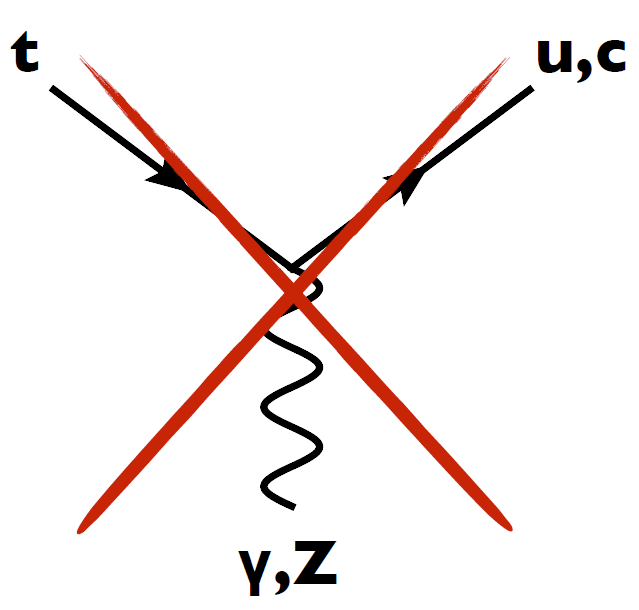
\includegraphics[width=0.2 \textwidth]{FCNC_SM.png}
\hspace{1cm}
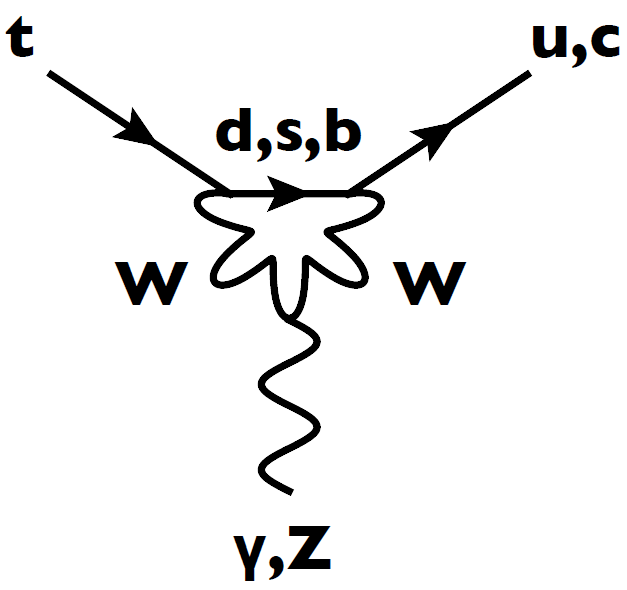
\includegraphics[width=0.2 \textwidth]{FCNC_SM_loop.png}
\hspace{1cm}
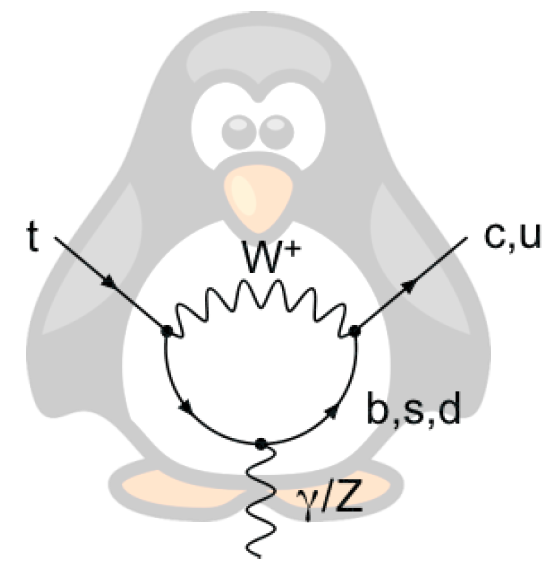
\includegraphics[width=0.2 \textwidth]{FCNC_SM_pin.png}
\]
           
\end{frame}

%------------------------------------------------
\begin{frame}
	\frametitle{Experimental Limits}
%	\framesubtitle{and a subtitle!}
%\footnotesize
\small
 \begin{itemize}
	\item LHC experiments have been searching for Top FCNC. 
	\item So far, \textcolor{Red}{no clear evidence for the presence of top quark FCNC interactions} has been observed and upper limits are set on the anomalous couplings and top quark branching.
	\end{itemize}
\begin{columns}
	\begin{column}{0.55\textwidth}
	\[\hspace{-1cm}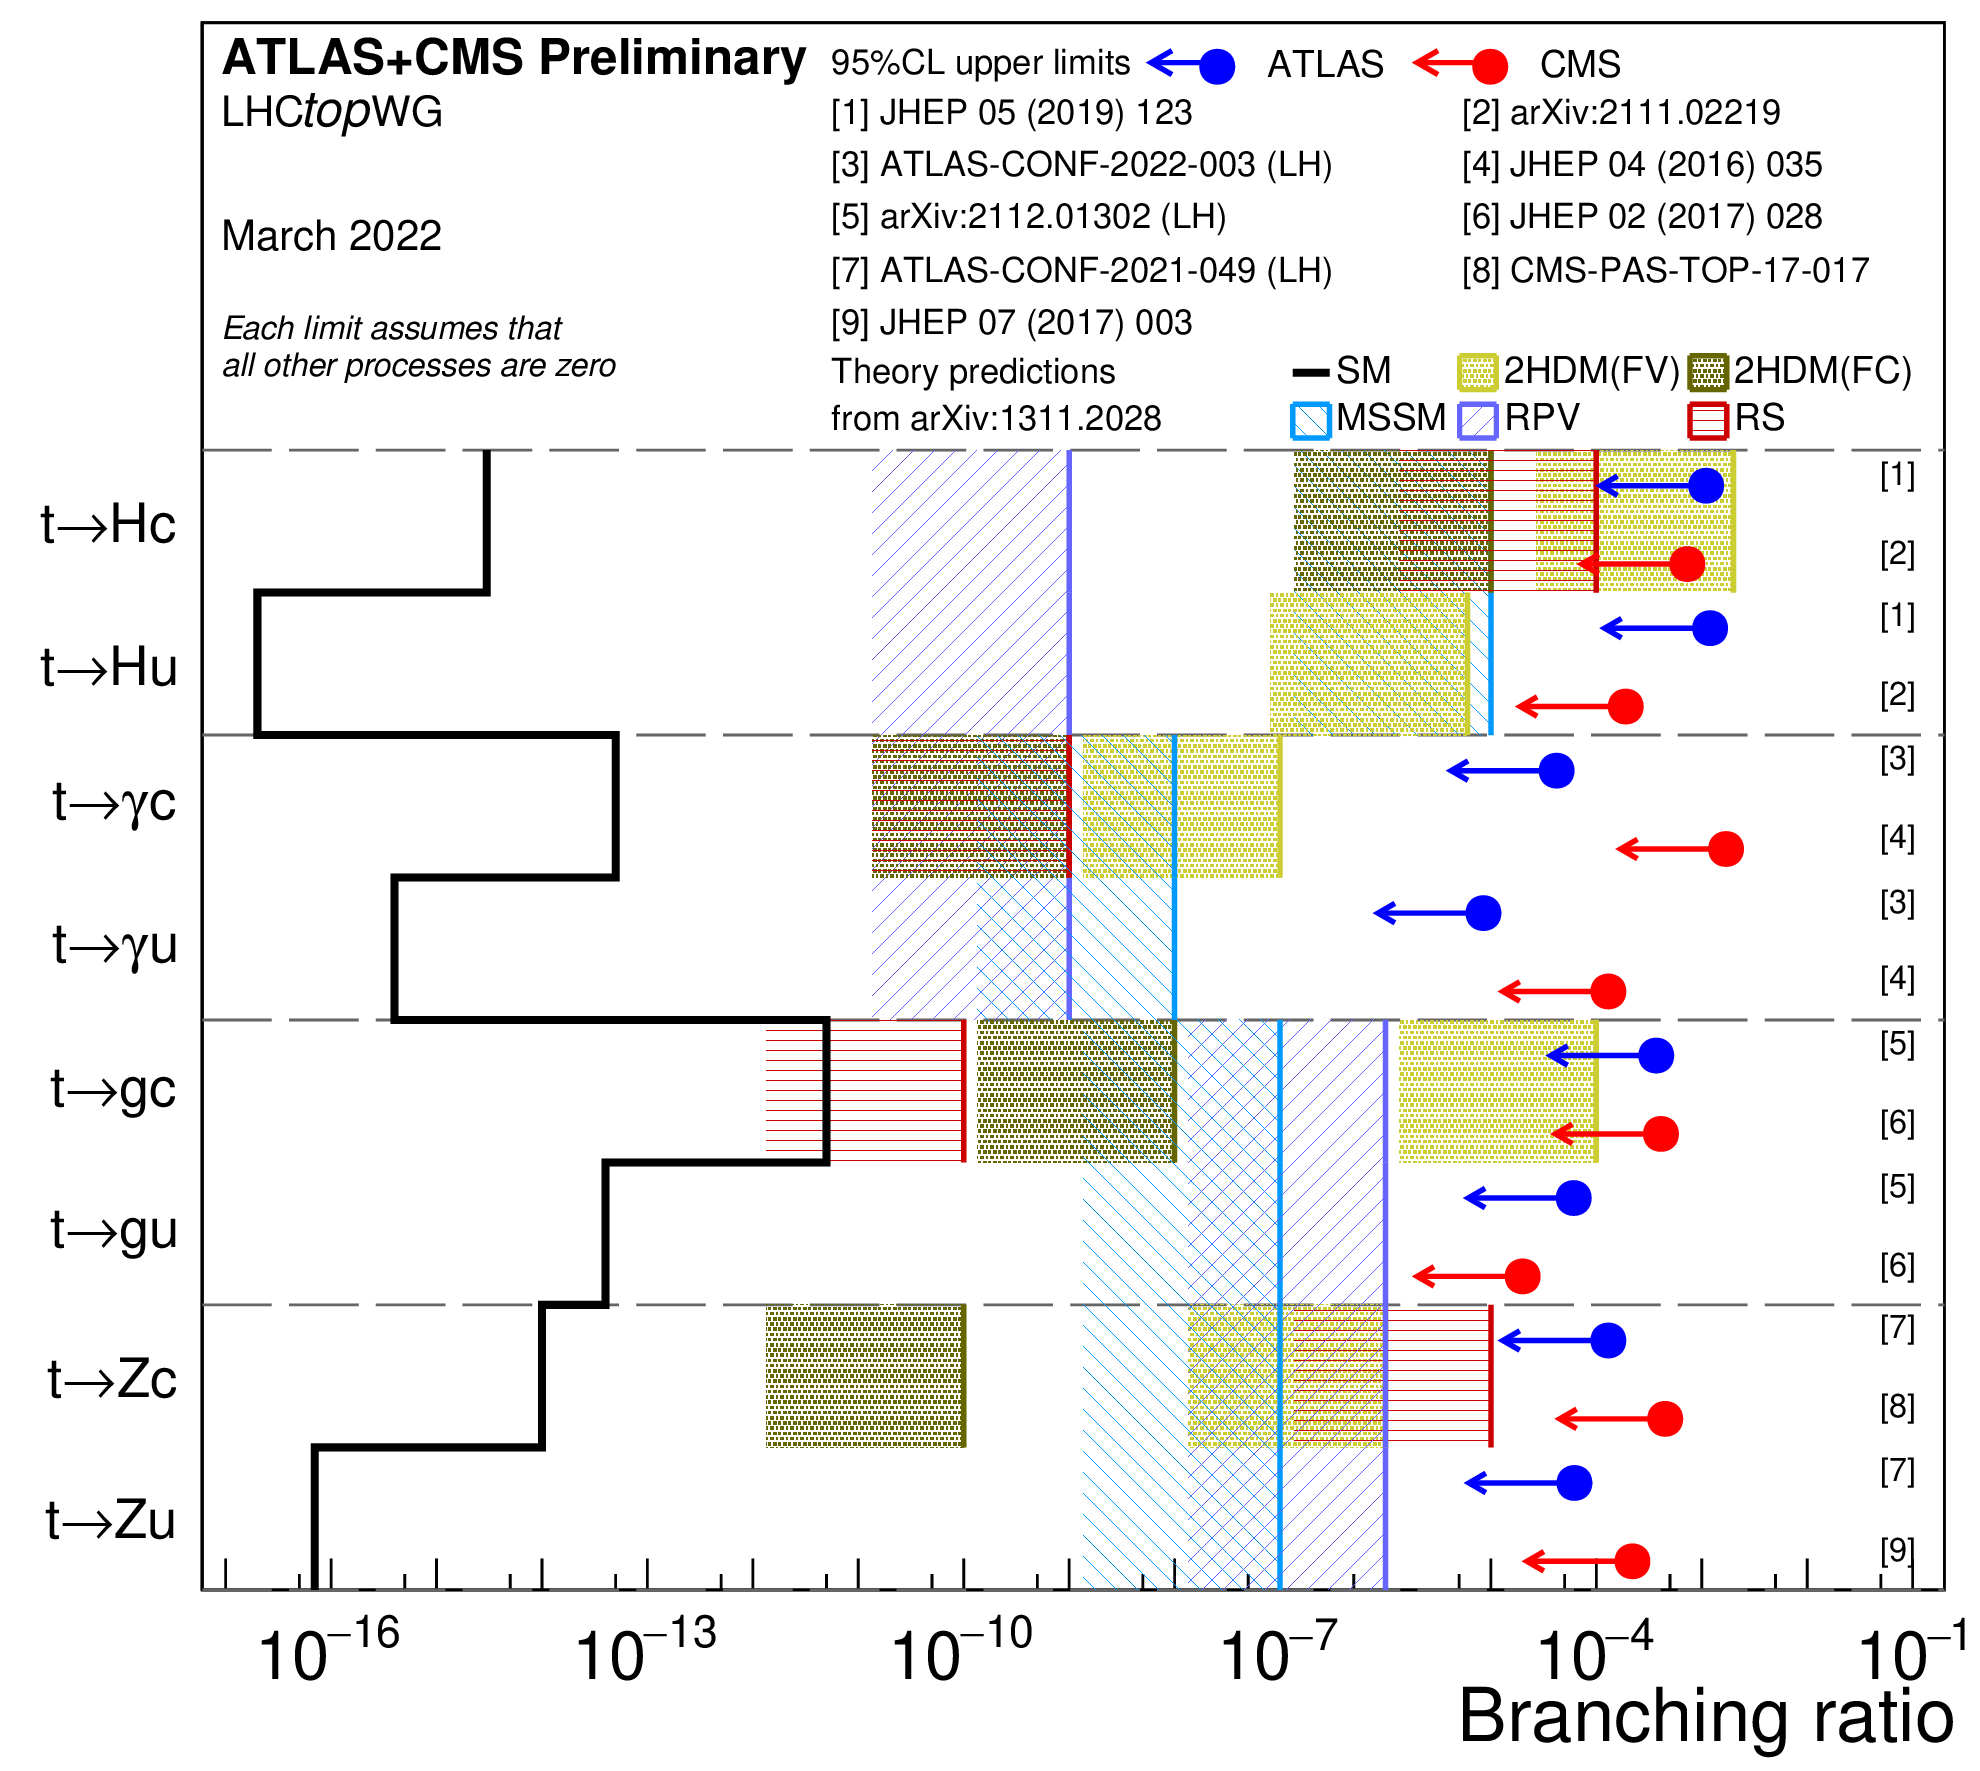
\includegraphics[width=0.68 \textwidth]{recent_limit_FCNC.png}\]
	\end{column}
	\begin{column}{0.44\textwidth}
		\[\hspace{-2cm}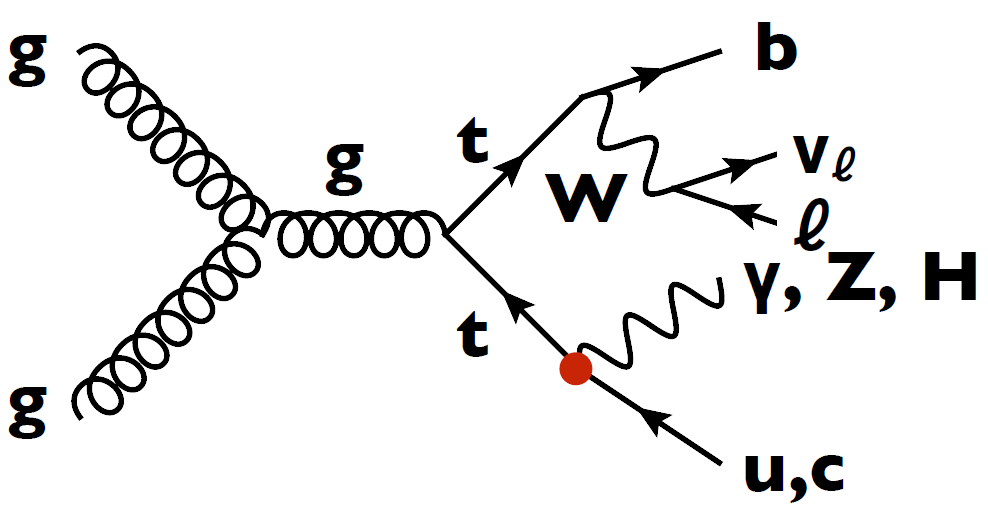
\includegraphics[width=0.43\textwidth]{feyn1.png}
	\hspace{0.5cm}	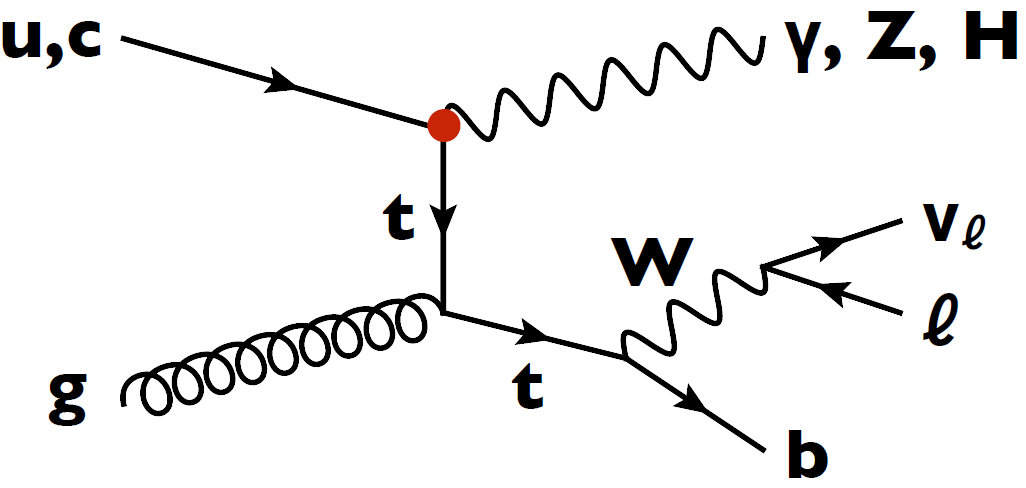
\includegraphics[width=0.43 \textwidth]{feyn2.png}
		%	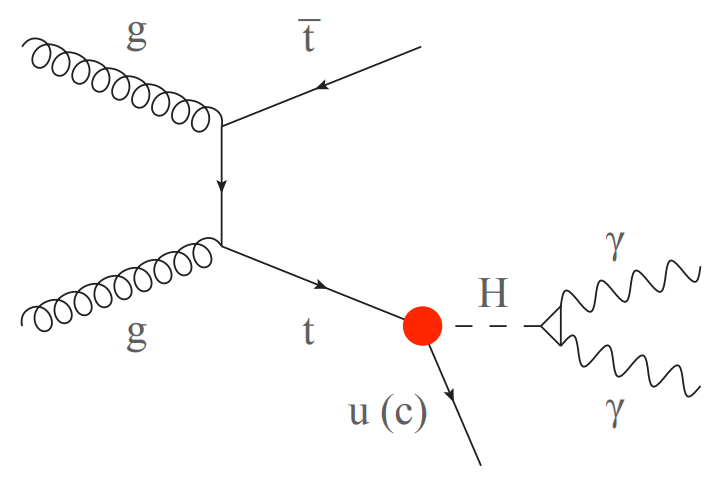
\includegraphics[width=0.43 \textwidth]{feyn4.png}
		\]
			\[\hspace{-3cm}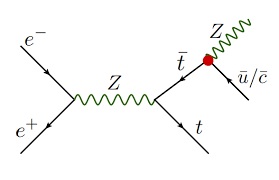
\includegraphics[width=0.44 \textwidth]{FCNC_tt.png}
			\hspace{0.5cm}
			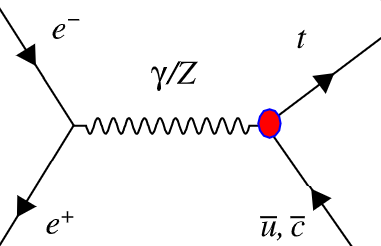
\includegraphics[width=0.43 \textwidth]{feyn1_SM_ee.png}\]
\end{column}
\end{columns}	
 \begin{itemize}
	\item OPAL $\&$ {\bf 600 pb$^{-1}$} data collected at {\bf 189-209 GeV} $\&$ leptonic and the hadronic decay modes of the W boson $\&$ the Durham algorithm [{\it Physics Letters B 521 (2001)} 181-194]($Br(t\rightarrow zq)=13.7 \%$).
	
   \item	L3 $\&$ {\bf the total integrated luminosity of  634 pb$^{-1}$} $\&$ {\bf $\sqrt{s}=$189 to  209 GeV } $\&$ Durham algorithm [{\it Physics Letters B 549 (2002) 290-300}]  ($Br(t\rightarrow \gamma q)=4.1 \%$ and $Br(t\rightarrow Z q)=13.7 \%$).
\end{itemize}


\end{frame}

\section{Top-FCNC appearance at FCC-ee }
%------------------------------------------------
\begin{frame}
\efboxsetup{linecolor=green,linewidth=2pt}
	\frametitle{Effective Framework}
	The most general effective Lagrangian describing the FCNC interactions can be parameterized as:
	
         \[ \efbox{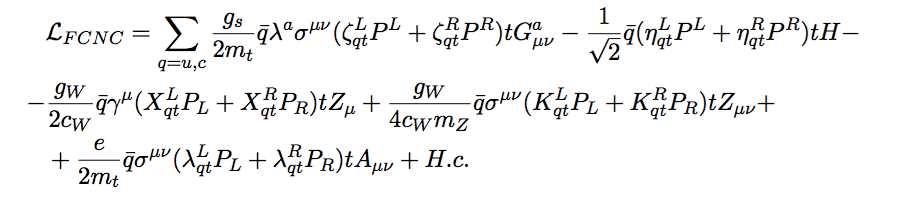
\includegraphics[width=0.8 \textwidth]{lfcnc.png}}\] 
          \[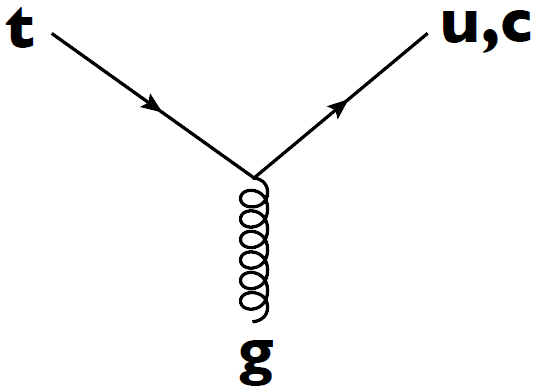
\includegraphics[width=0.2 \textwidth]{vertex1.png}
          \hspace{1cm}
          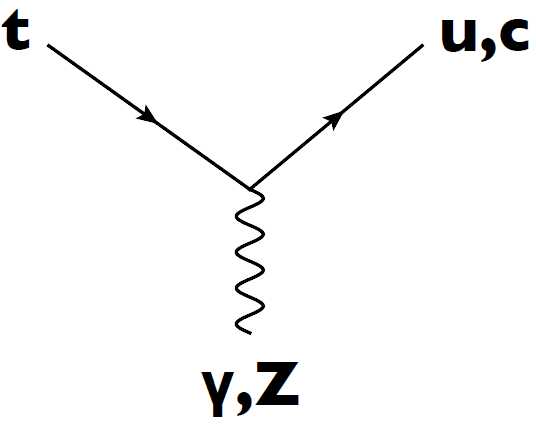
\includegraphics[width=0.2 \textwidth]{vertex2.png}
           \hspace{1cm}
           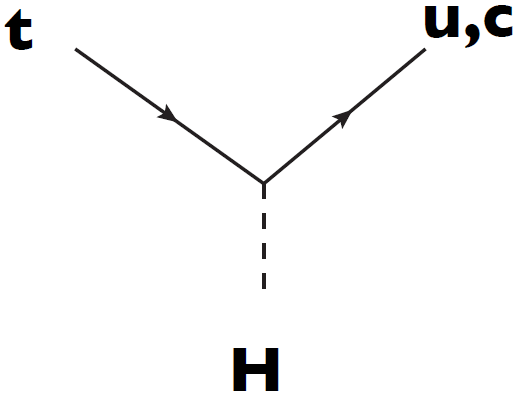
\includegraphics[width=0.2 \textwidth]{vertex3.png}\]
           \centering
           \vspace{1cm}
          \textcolor{red}{$\zeta_{qt}^{L} =  \zeta_{qt}^{R}$ ~~~~~~~~~~~  
          $\eta_{qt}^{L} =  \eta_{qt}^{R}$~~~~~~~~~~~ $\kappa_{qt}^{L} =  \kappa_{qt}^{R}$~~~~~~~~~~~  
          $X_{qt}^{L} =  X_{qt}^{R}$~~~~~~~~~~~
           $\lambda_{qt}^{L} =  \lambda_{qt}^{R}$}
\end{frame}
\section{Analysis strategy}
%------------------------------------------------
\begin{frame}
\label{Test} %For the link button for the Appendix slide
	\frametitle{FCNC production at FCC-ee}
	\begin{columns}[t] % The "c" option specifies centered vertical alignment while the "t" option is 
	\begin{column}{0.5\textwidth} % Right column width
	\begin{itemize}
		\item At the FCCee, FCNC $tqV$  interaction can lead to
		single top production
		
		\item	This analysis is performed  at  the center of mass energy
		240 and 365 GeV.
		
		\item	The distinctive signature of the signal is:
		\begin{itemize}
		\item A top quark
		\item  A light energetic jet
		\end{itemize}
	\end{itemize}
		
	\end{column}
	\begin{column}{0.5\textwidth} % Left column width
		\begin{figure}[h!]
			\centering
			\vspace{-0.5cm}
			\[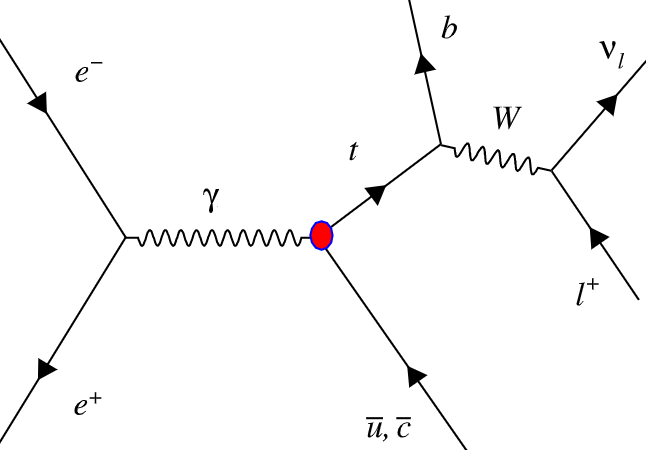
\includegraphics[width=0.7 \textwidth]{Feyn.png}\]
		\end{figure}
	\textcolor{purple}{{\bf signal signature:}} One lepton, one neutrino, exactly 2exclusive jets which one of them are tagged as b-jet.
	\end{column}		
\end{columns}
\vspace{0.5cm}
\textcolor{Blue}{
 All MC files are generated in the FCCSW (https://github.com/HEP-FCC/FCCAnalyses) framework with $DelphesPythia8_EDM4HEP$ and IDEA Delphes Card}
\end{frame}
%%%%%%%%%%%%%%%%%%%%%%%%%%%%%%%%%%5
\begin{frame}
\frametitle{Jet clustering algorithms selection}
\small


	\begin{columns}[t] % The "c" option specifies centered vertical alignment while the 
			\begin{column}{0.5\textwidth} % Right column width
				\centering
				 Exactly two  exclusive jet is required:
	\[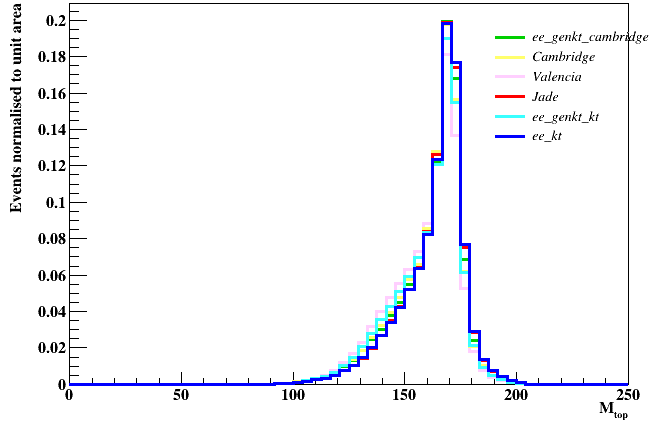
\includegraphics[width=0.8\textwidth]{jet_Alg_mtop.png}\]
	%\[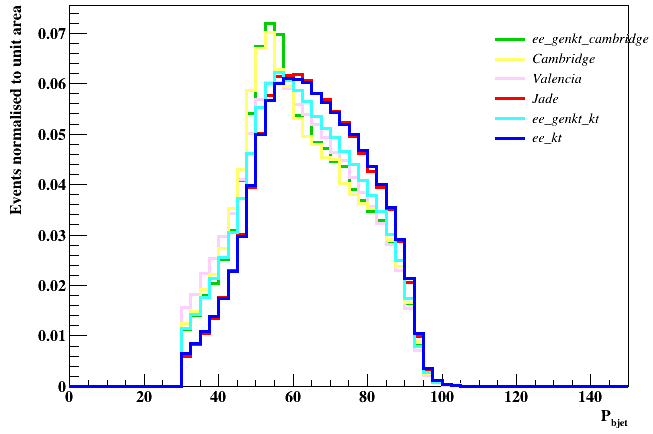
\includegraphics[width=0.73 \textwidth]{jet_Alg_pbjet.png}\]

	\end{column}
	\begin{column}{0.5\textwidth} % Left column width
		Reconstructed top mass distribution for three different schemes, for $tc\gamma$ coupling.
	%	\begin{figure}[h!]
			%\centering
		%	\vspace{-0.5cm}
			\[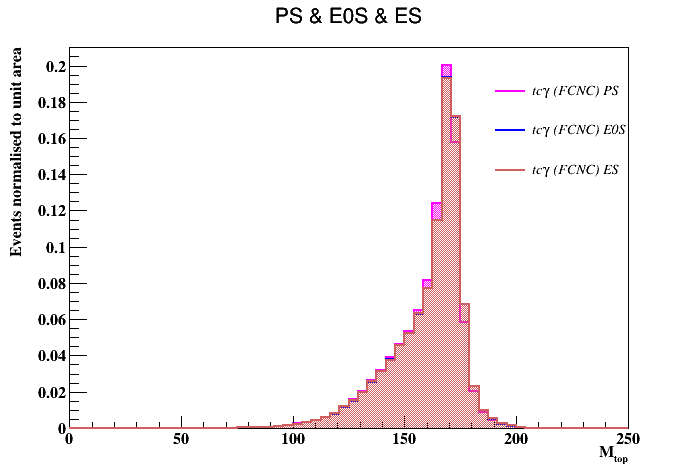
\includegraphics[width=0.8 \textwidth]{Rec_scheme.png}\]
	%	\end{figure}
	
	\end{column}		
\end{columns}
\centering
	\vspace{0.5cm}
\textcolor{red}{\bf Jet Definition = Durham $\&$ E-scheme}  
\end{frame}

%------------------------------------------------
\subsection{signal selection and Background estimation}

%------------------------------------------------
\begin{frame}
\label{Test Stat}
\frametitle{MC simulation}

\begin{columns}
	\hspace{1cm}
	\begin{column}{0.3\textwidth} % Right column width
		\scalebox{0.8}{
			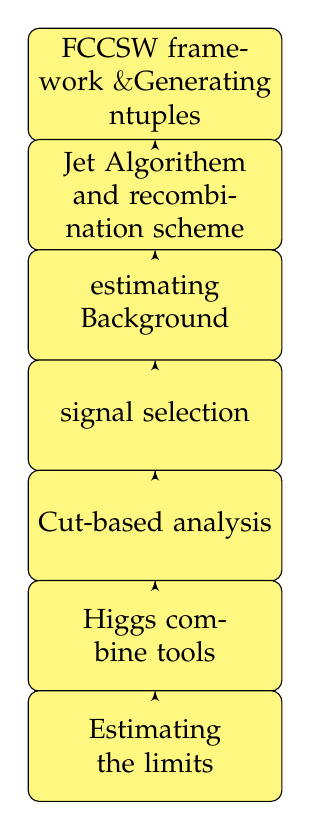
\begin{tikzpicture}[node distance = 1.4cm, auto] 
			\node [block] (init) {FCCSW framework $\&$Generating ntuples};  
			\node [block, below of= init](ReadA){Jet Algorithem and recombination scheme};  
			\node [block, below of= ReadA](ReadB){estimating Background};  
			\node [block, below of = ReadB](Sum){signal selection};  
			\node [block, below of = Sum](P){Cut-based analysis};  
		   \node [block, below of = P](P2){Higgs combine tools};  
			\node [block, below of = P2](Out){Estimating the limits};  
			\path [line] (init) -- (ReadA);   
			\path [line] (ReadA) -- (ReadB);   
			\path [line] (ReadB) -- (Sum);   
		    \path [line] (Sum) -- (P);   
			\path [line] (P) -- (P2);   
			\path [line] (P2) -- (Out);   
			
			\end{tikzpicture}  
		}
	\end{column}
	
	\begin{column}{0.5\textwidth} % Right column width
		{\bf Backgrounds:}
		\setbeamercolor{coloredboxstuff}{fg=black,bg=blue!10!white}
		\begin{beamercolorbox}[wd=1\textwidth,sep=1em]{coloredboxstuff}
			
			\scalebox{0.9}{
				\begin{tabular}{c|c|c}
					\hline
					
					& $\sigma$[fb]&  $\sigma$[fb]\\
					\hline
					Process~& $\sqrt{s}=240$GeV & $\sqrt{s}=365$GeV \\
					\hline
					$ZH$ & $202$& $117$ \\
					$WW$ &$16439$& $10717$\\
					$ZZ$& $1360$& $643$\\
					$e^-e^+q\bar{q}$ &$1637$&$620$  \\
					single top &$ 0.01$&$0.2$  \\
					$tbjj$ &-&$6$\\
					$t\bar{t}$ &-&$800$\\
					\hline
					
					\end{tabular}%
				}
				\end{beamercolorbox}
				{\bf  preselection cuts:}
				\begin{itemize}
				\item Lepton and jets momentum are  required to have: $p>15$GeV
				\item Polar angle of lepton and jets are required to be: $\theta>13$ degree
				\item The angular separation between lepton and jets are required to satisfy: $\Delta R>0.5$
				\item Missing energy  is grather than 15 GeV
				\end{itemize}
				\end{column}
				\end{columns}
				\end{frame}

%----------------------------------------------
\begin{frame}{Mass reconstruction in electron and muon channels-240 GeV}
\hspace{2cm}\textcolor{red}{electron channel} \hspace{3cm} \textcolor{red}{muon channel}
	\[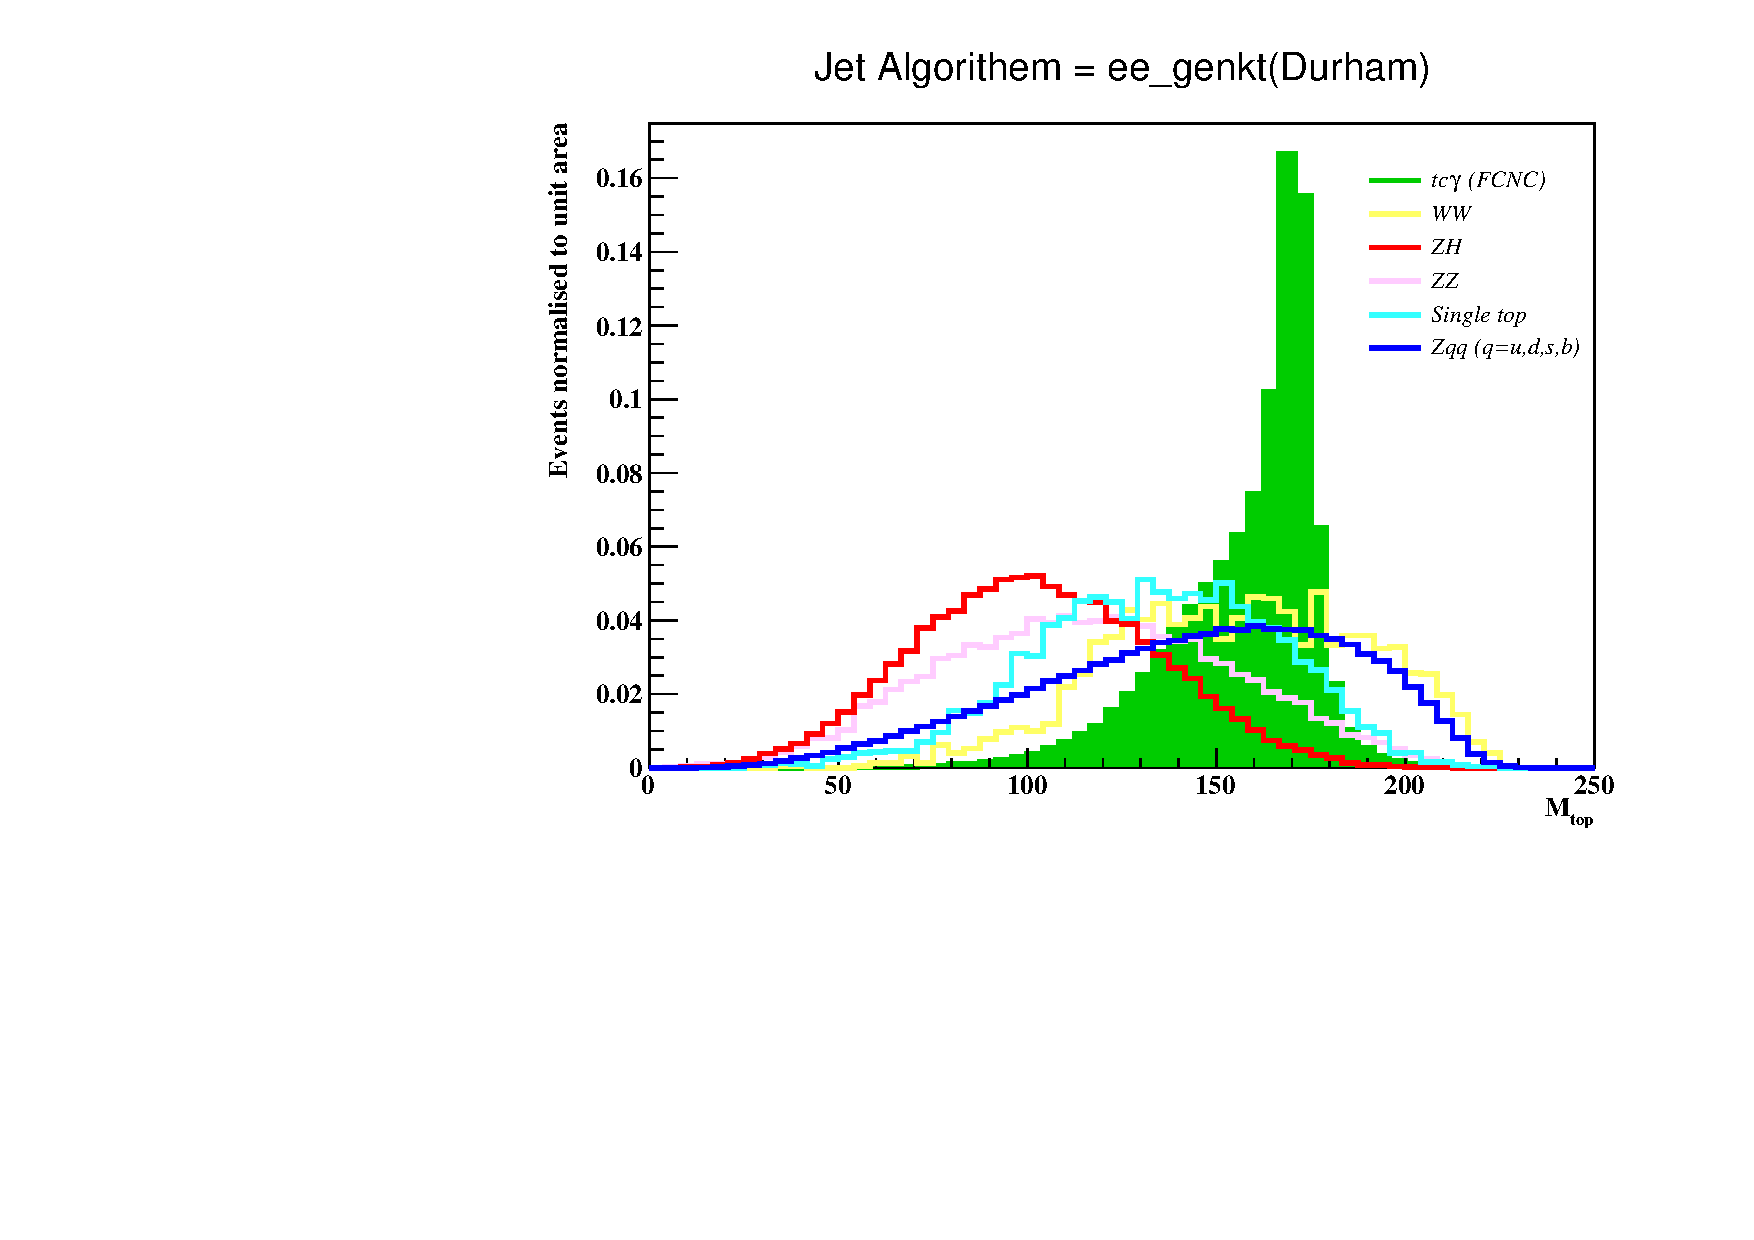
\includegraphics[width=0.40 \textwidth]{Plots-240/mtop_electron_240.pdf}
     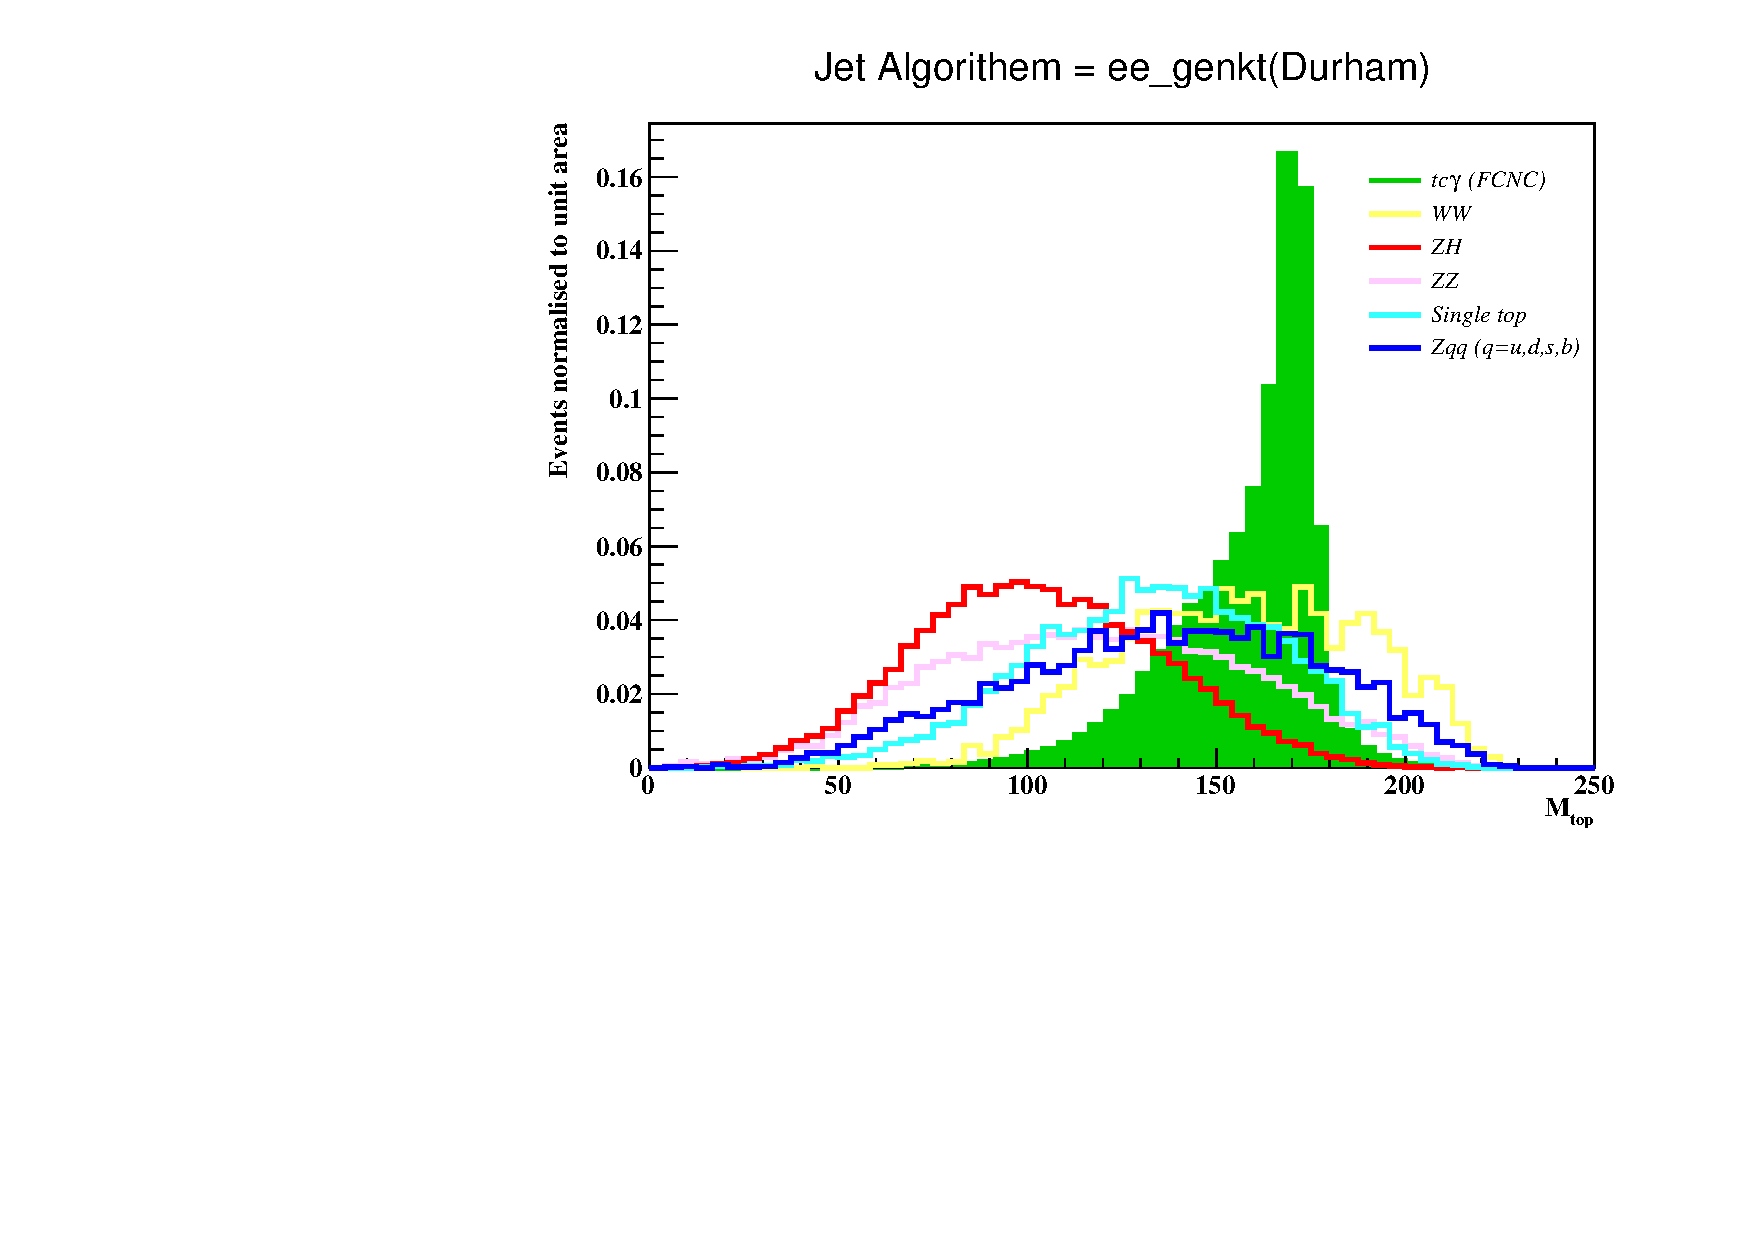
\includegraphics[width=0.40 \textwidth]{Plots-240/mtop_muon_240.pdf}
    \] 
    \[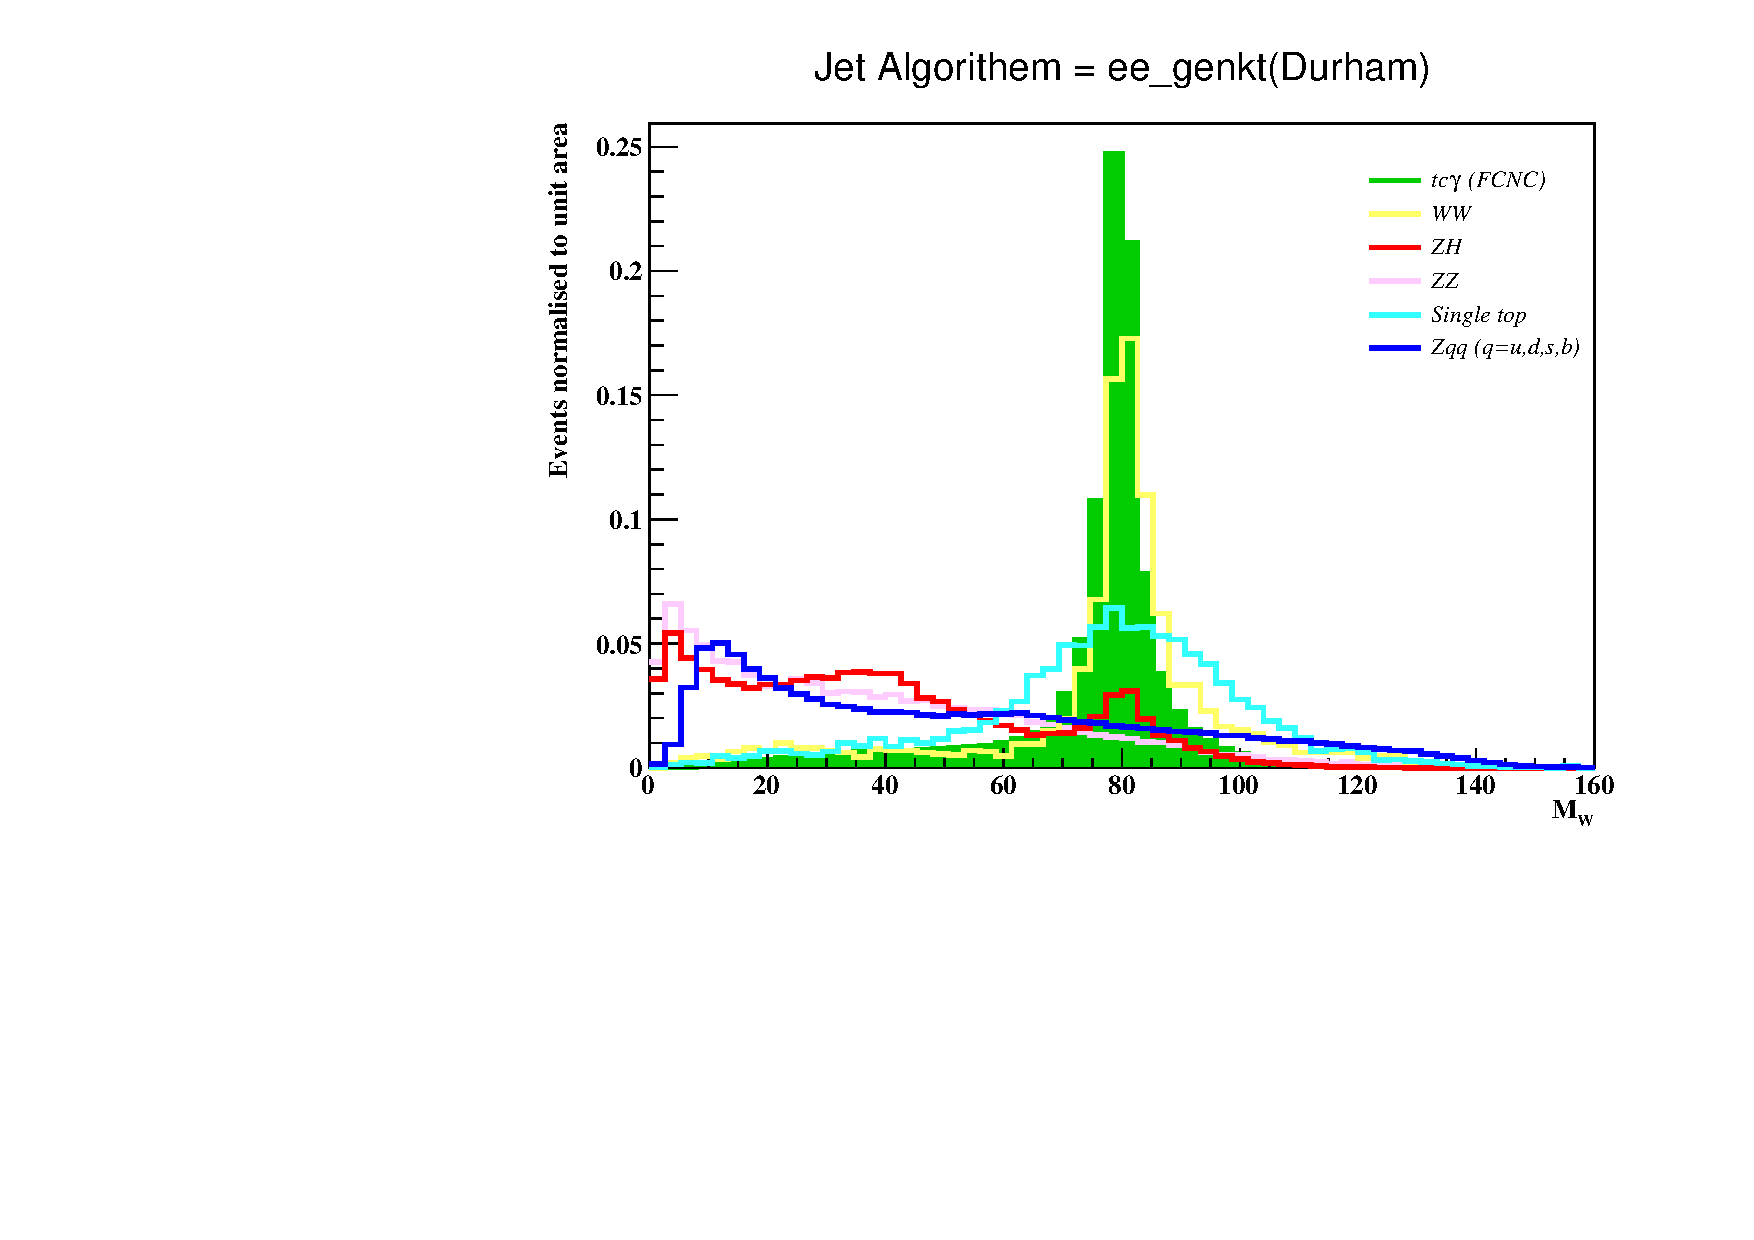
\includegraphics[width=0.40 \textwidth]{Plots-240/mW_electron_240.pdf}
    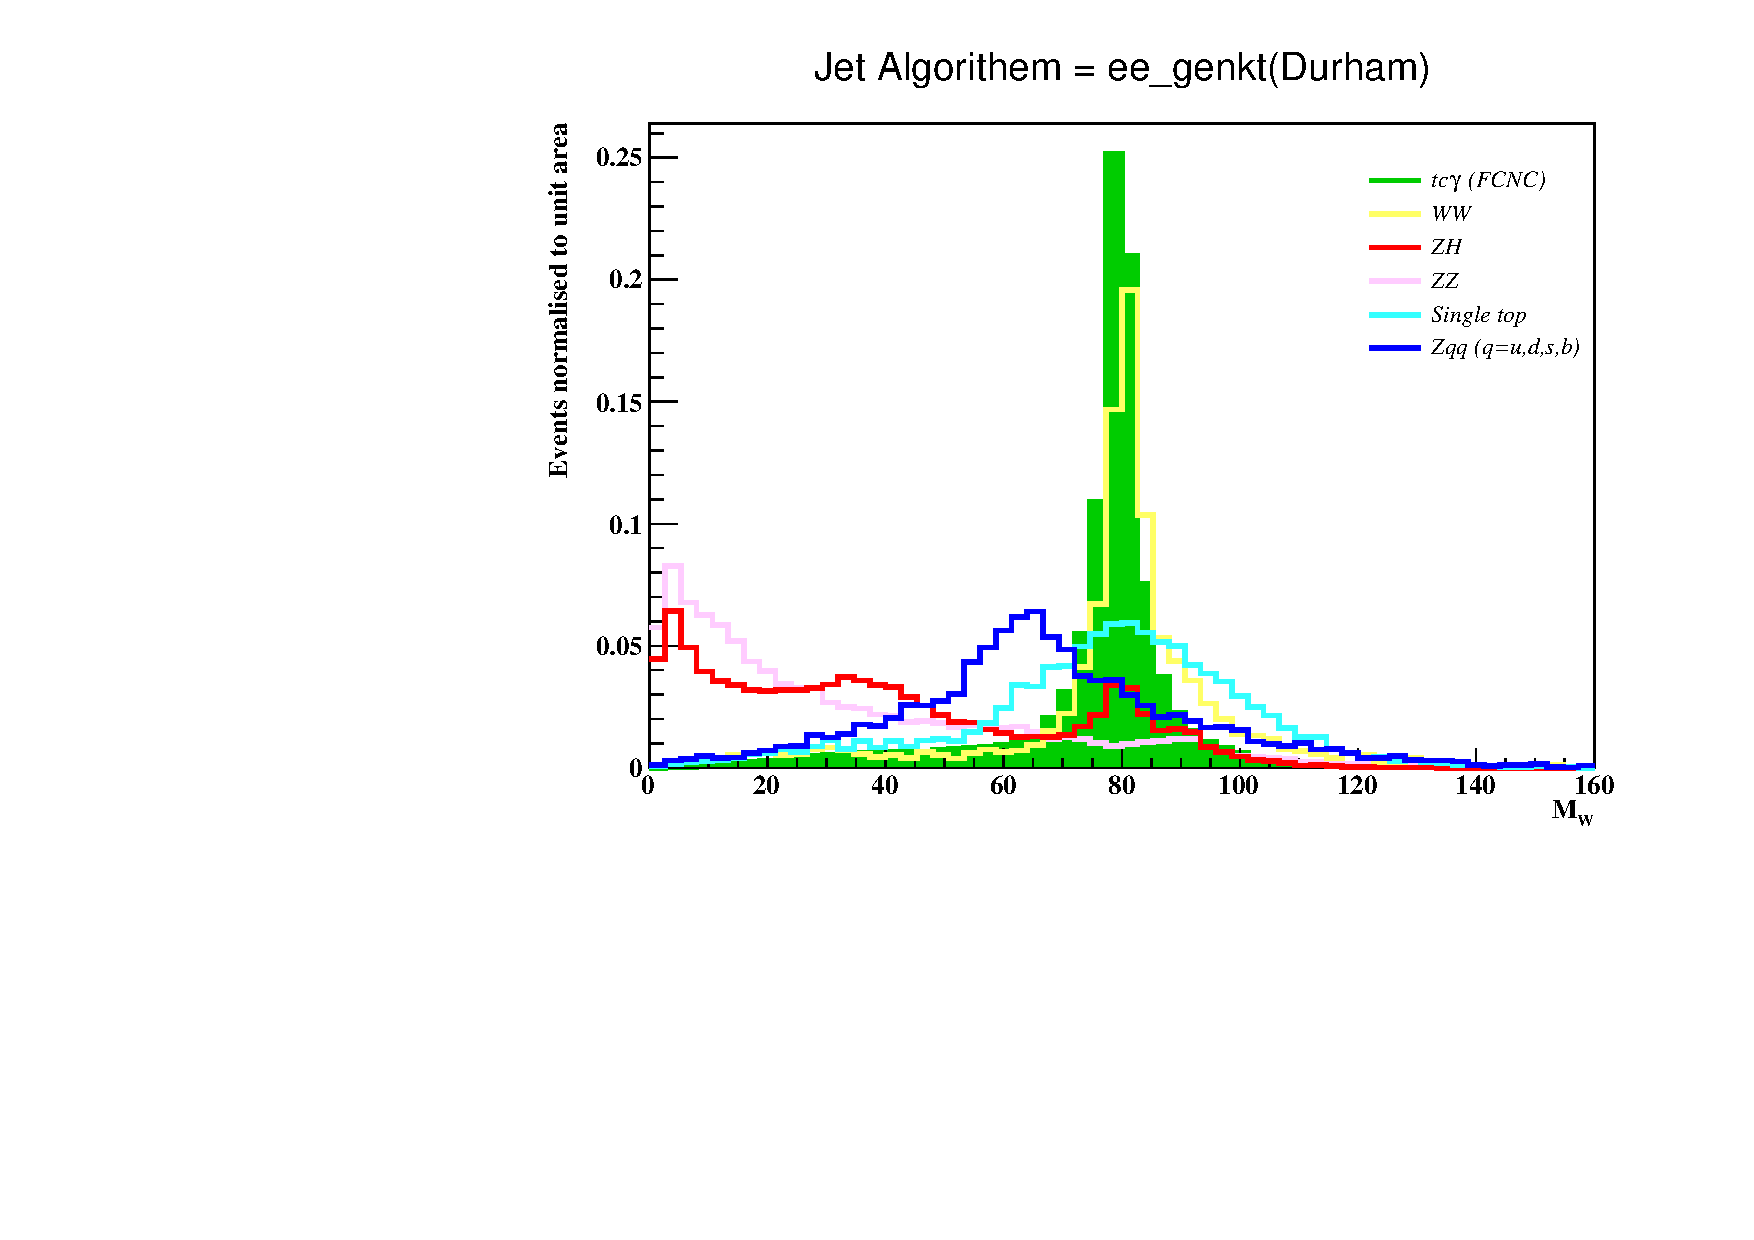
\includegraphics[width=0.40 \textwidth]{Plots-240/mW_muon_240.pdf}
    \] 
\end{frame}
\begin{frame}{Mass reconstruction in electron and muon channels-365 GeV}
\hspace{2cm}\textcolor{red}{electron channel} \hspace{3cm} \textcolor{red}{muon channel}
\[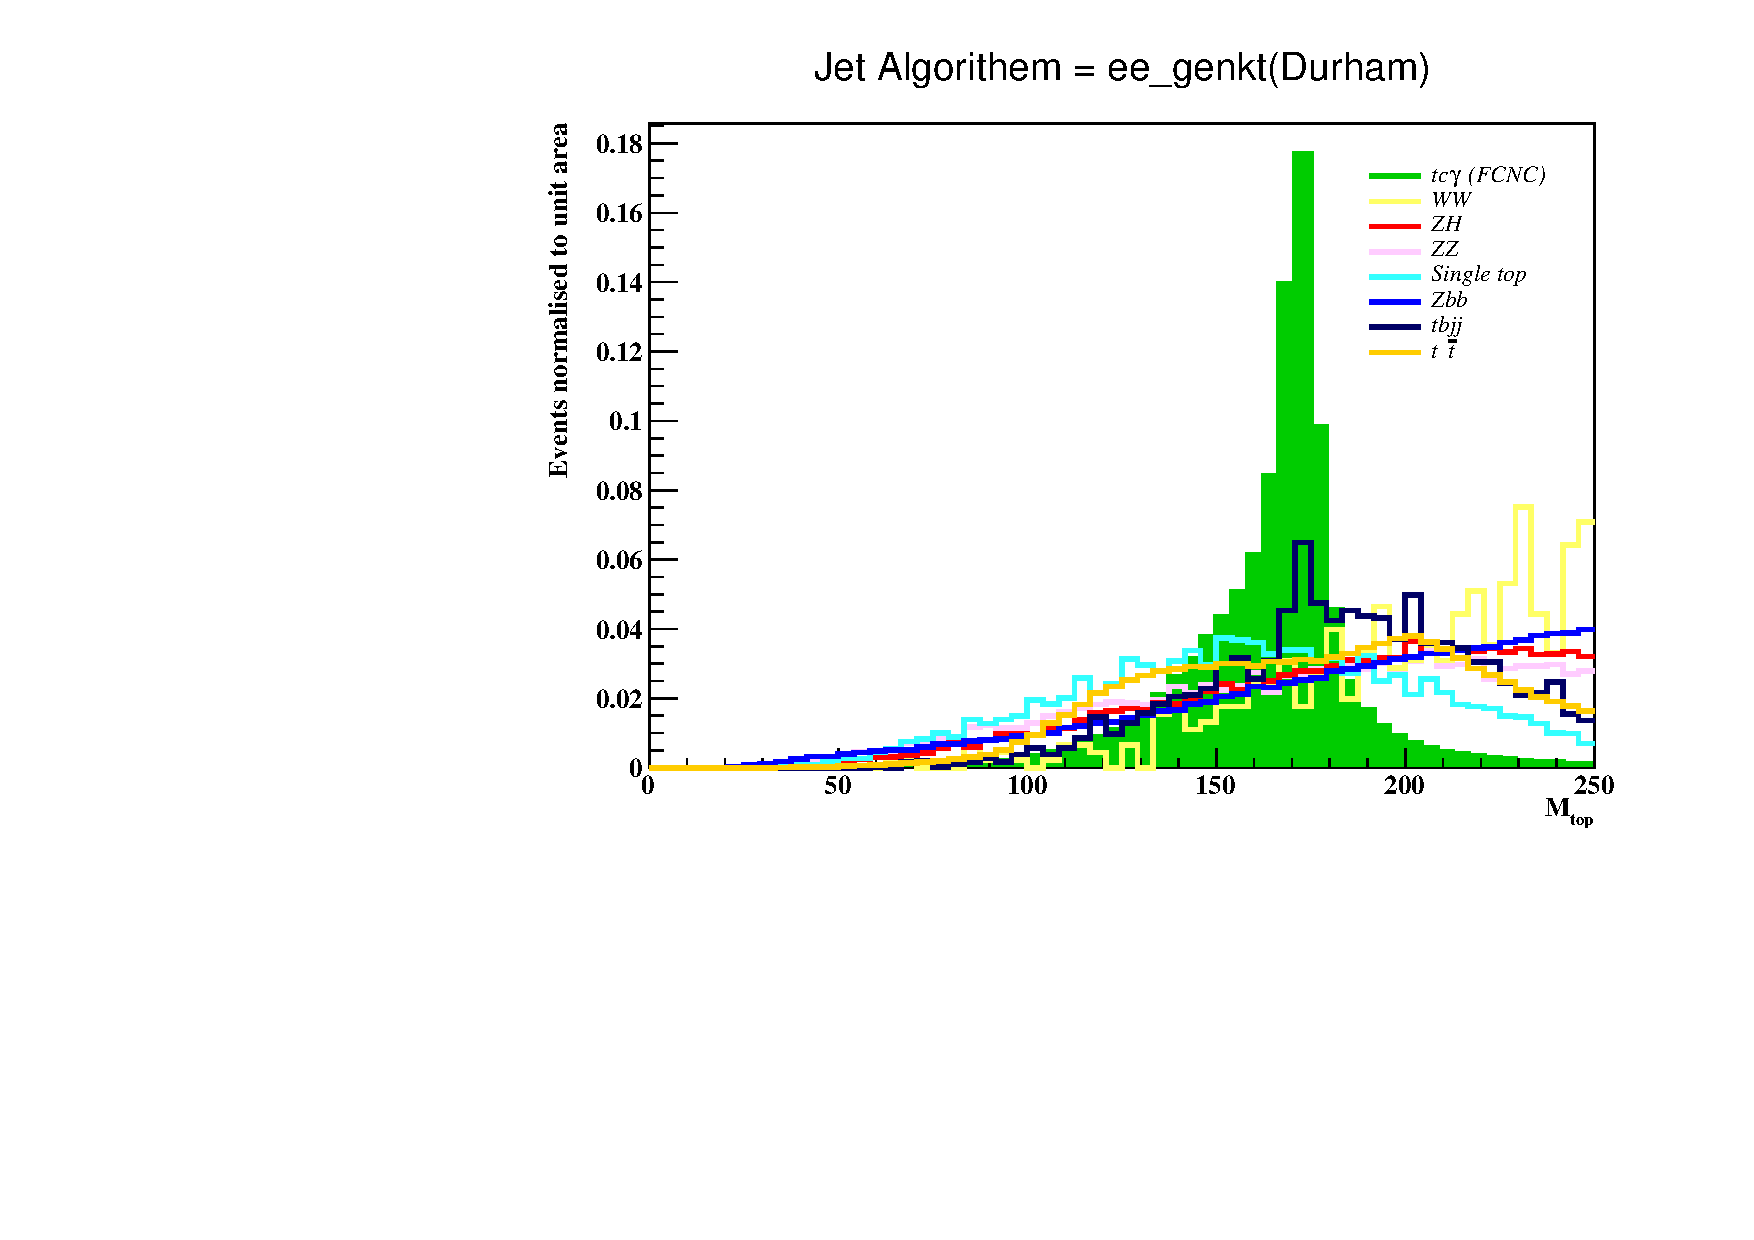
\includegraphics[width=0.40 \textwidth]{Plots-365/mtop_electron_365.pdf}
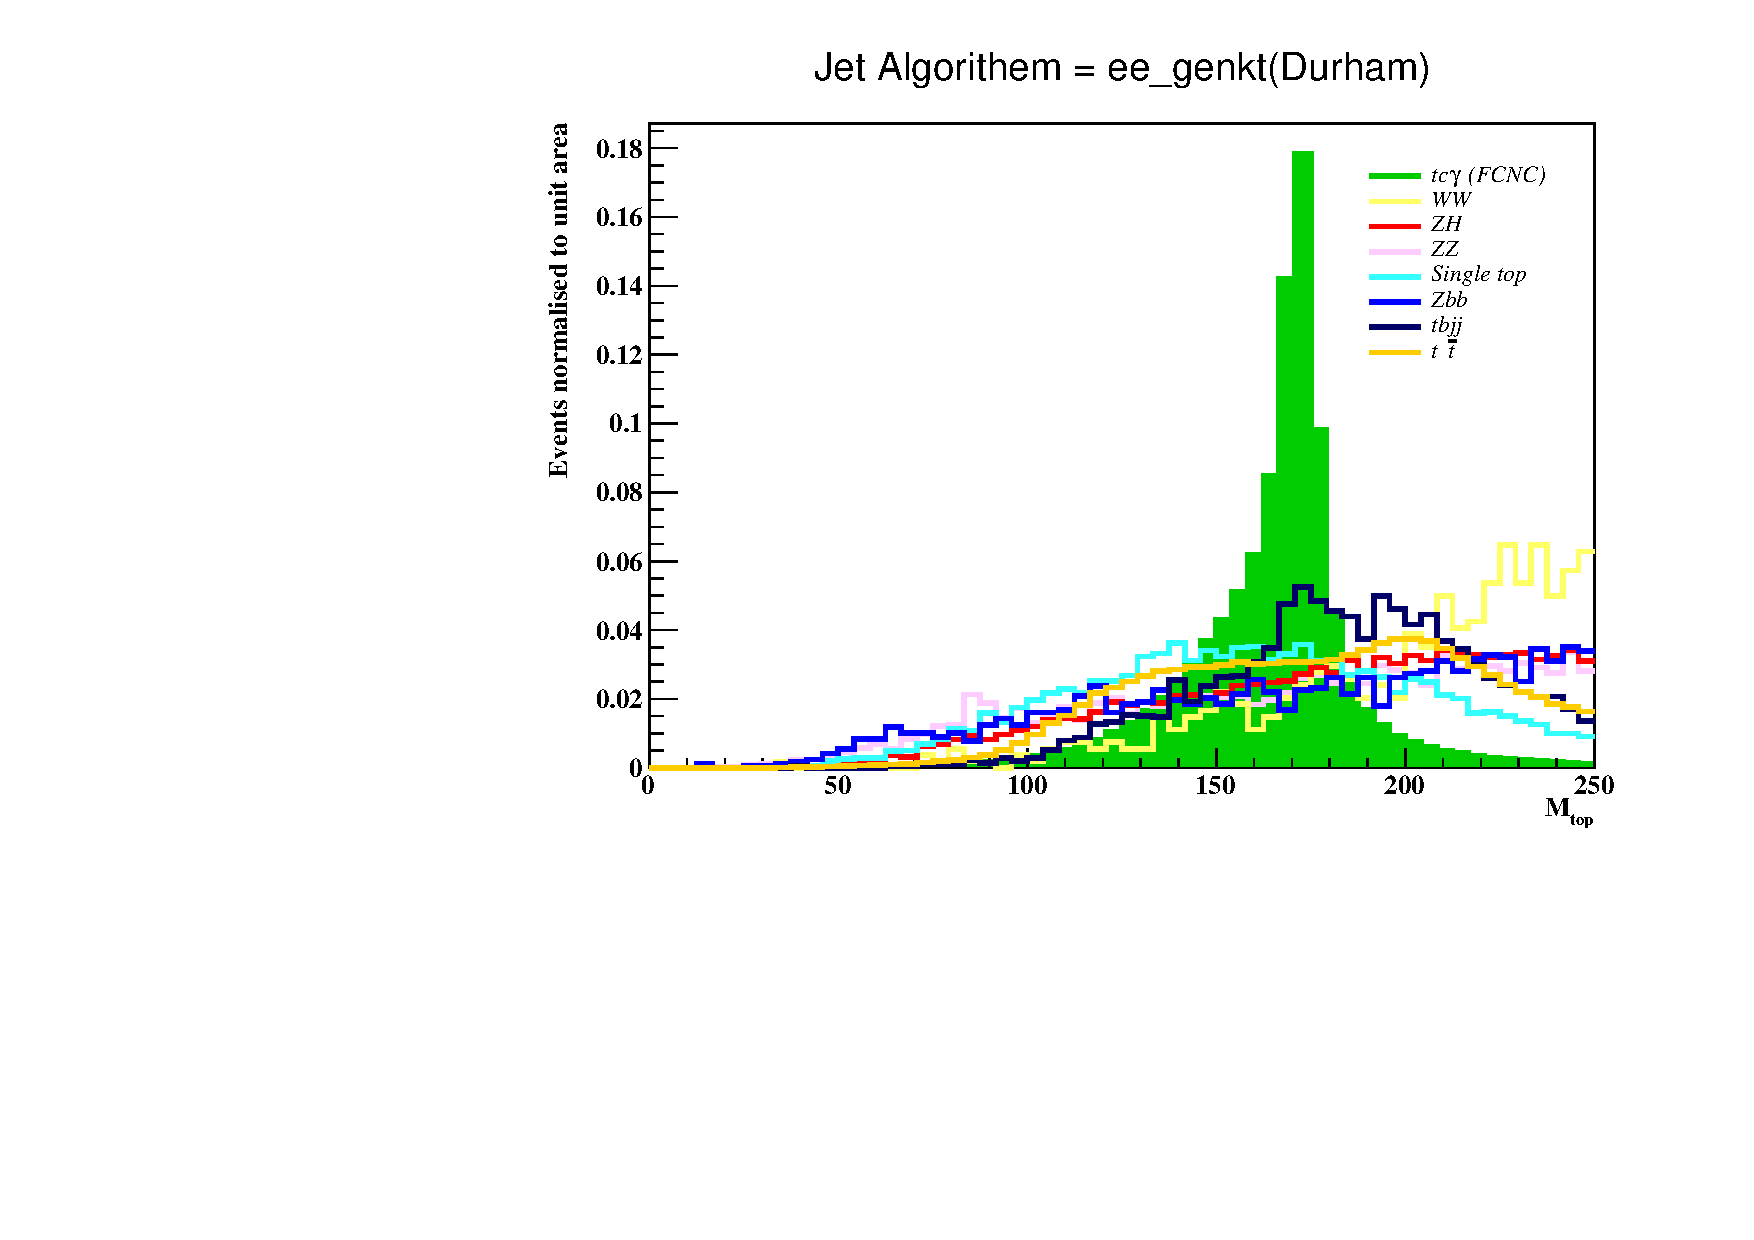
\includegraphics[width=0.40 \textwidth]{Plots-365/mtop_muon_365.pdf}
\] 
\[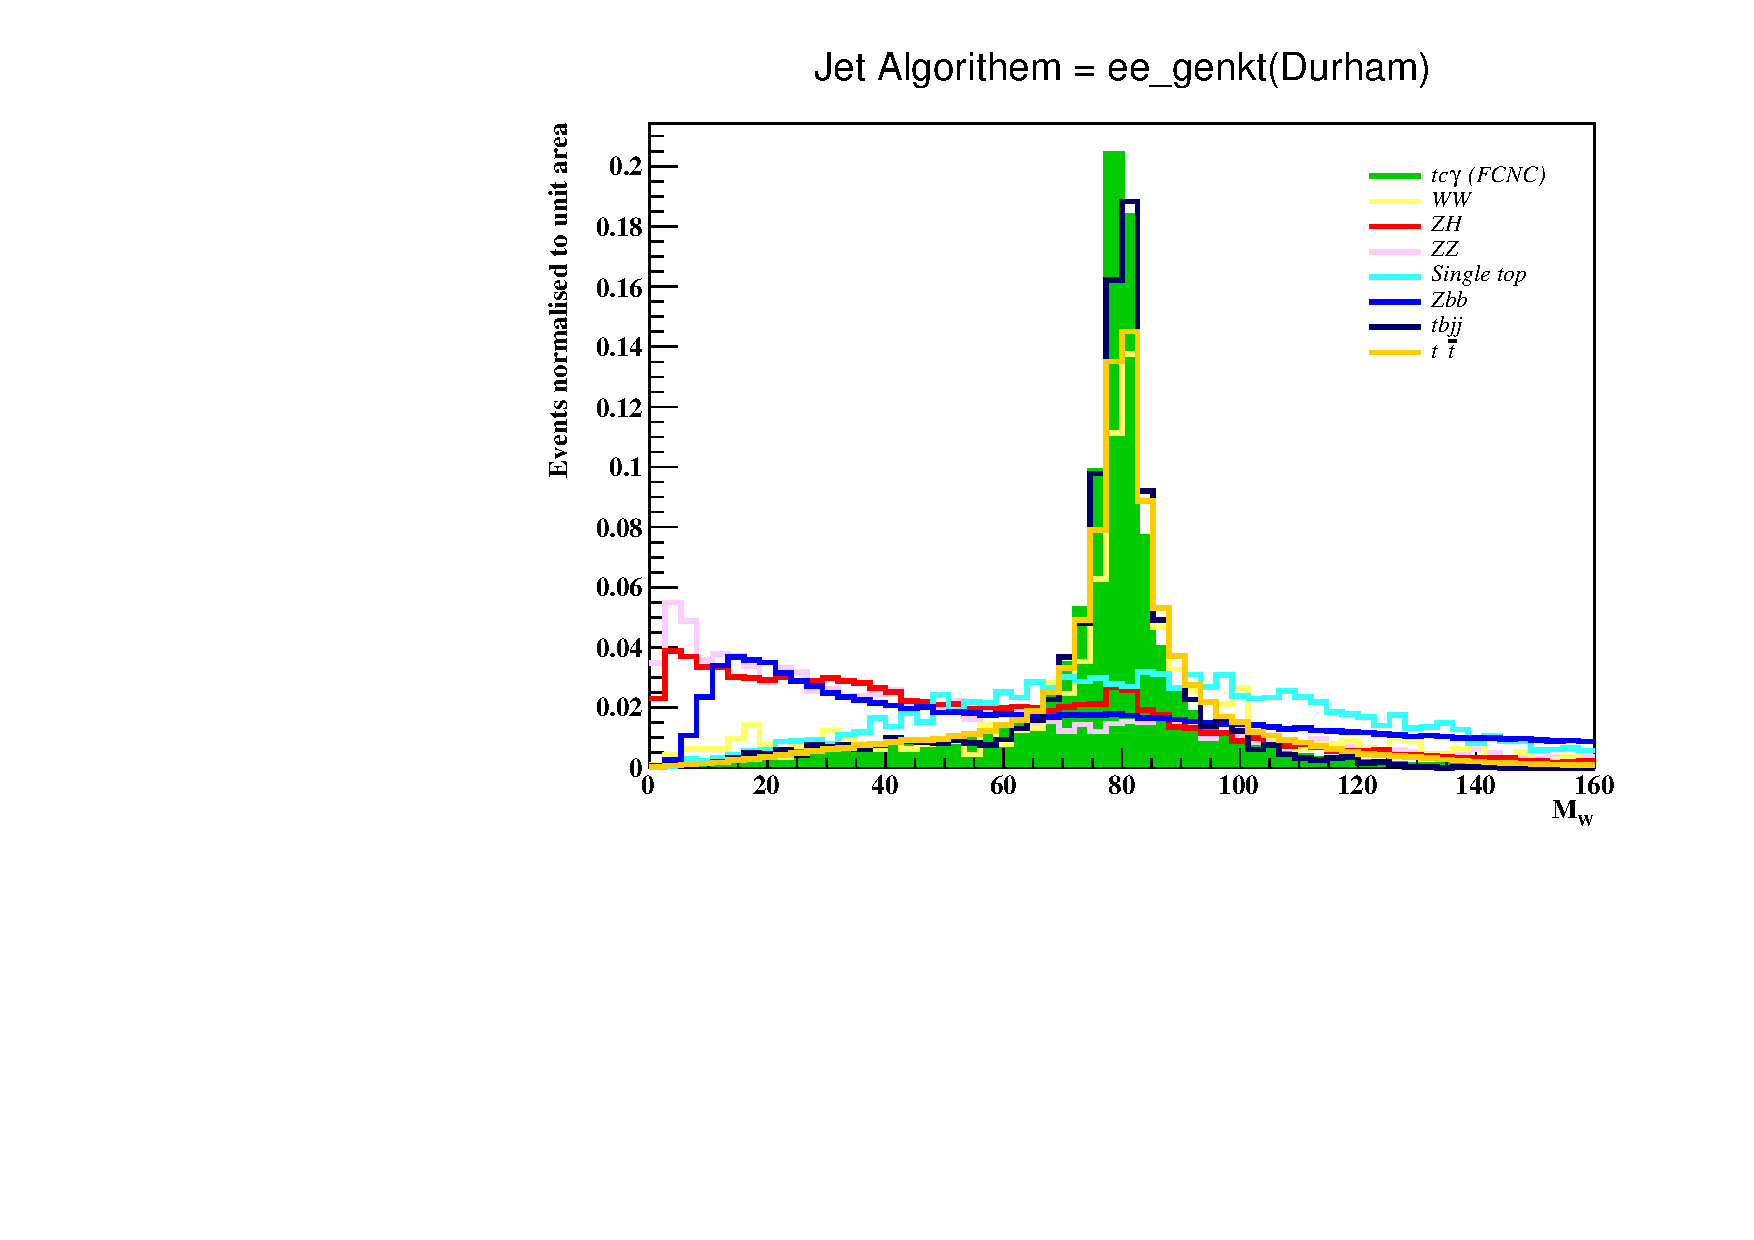
\includegraphics[width=0.40 \textwidth]{Plots-365/mW_electron_365.pdf}
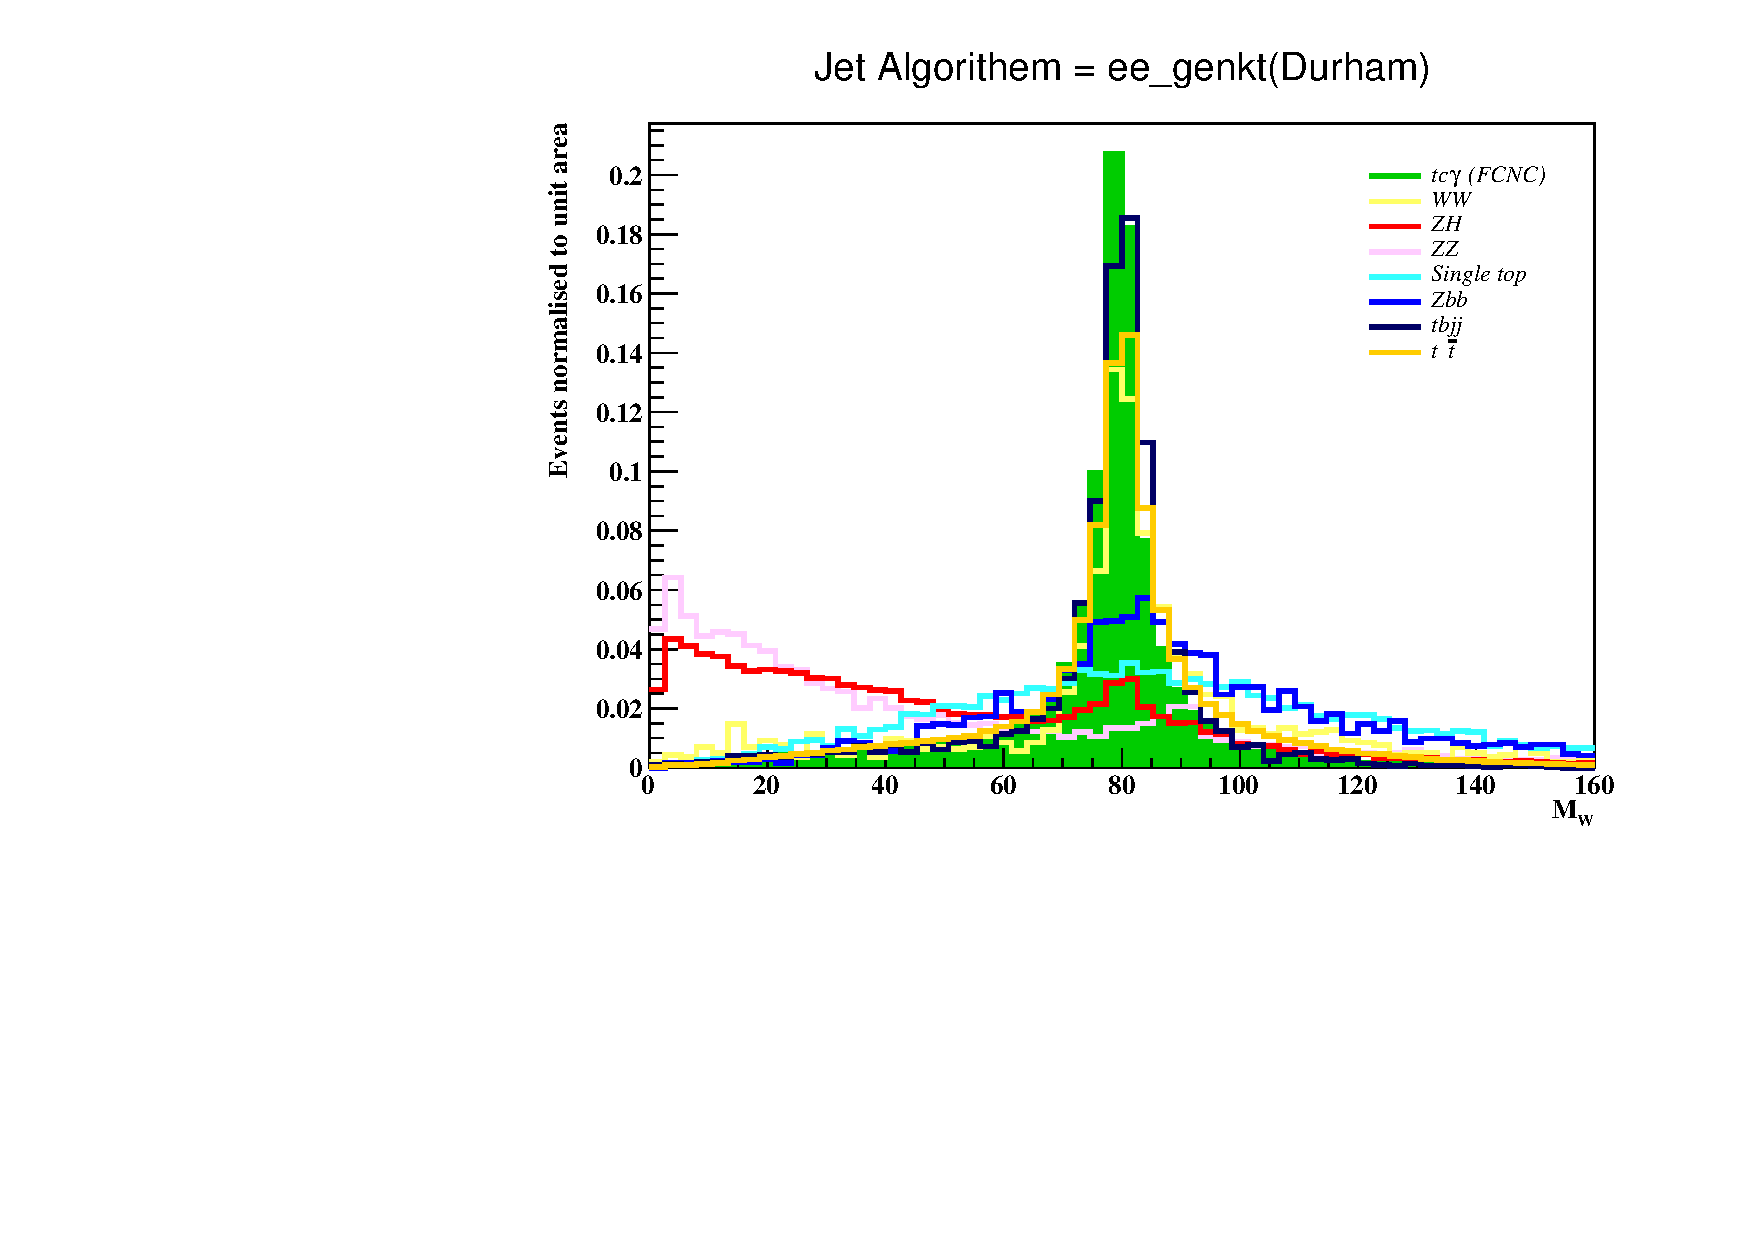
\includegraphics[width=0.40 \textwidth]{Plots-365/mW_muon_365.pdf}
\] 
\end{frame}
\begin{frame}{distinctive variables}

Optimal cuts on individual variables increase our sensitivity to the signal.
	\begin{columns}[t] % The "c" option specifies centered vertical alignment while the "t" option is 
	
	\begin{column}{0.2\textwidth} % Right column width
			\vspace{1.5cm} 	\hspace{3cm}
		\textcolor{red}{$\sqrt{s}=240$ GeV} \\
		\vspace{2cm} 	\hspace{3cm}
		\textcolor{red}{	$\sqrt{s}=365$ GeV }
	\end{column}
	\begin{column}{0.8\textwidth} % Left column width
	\[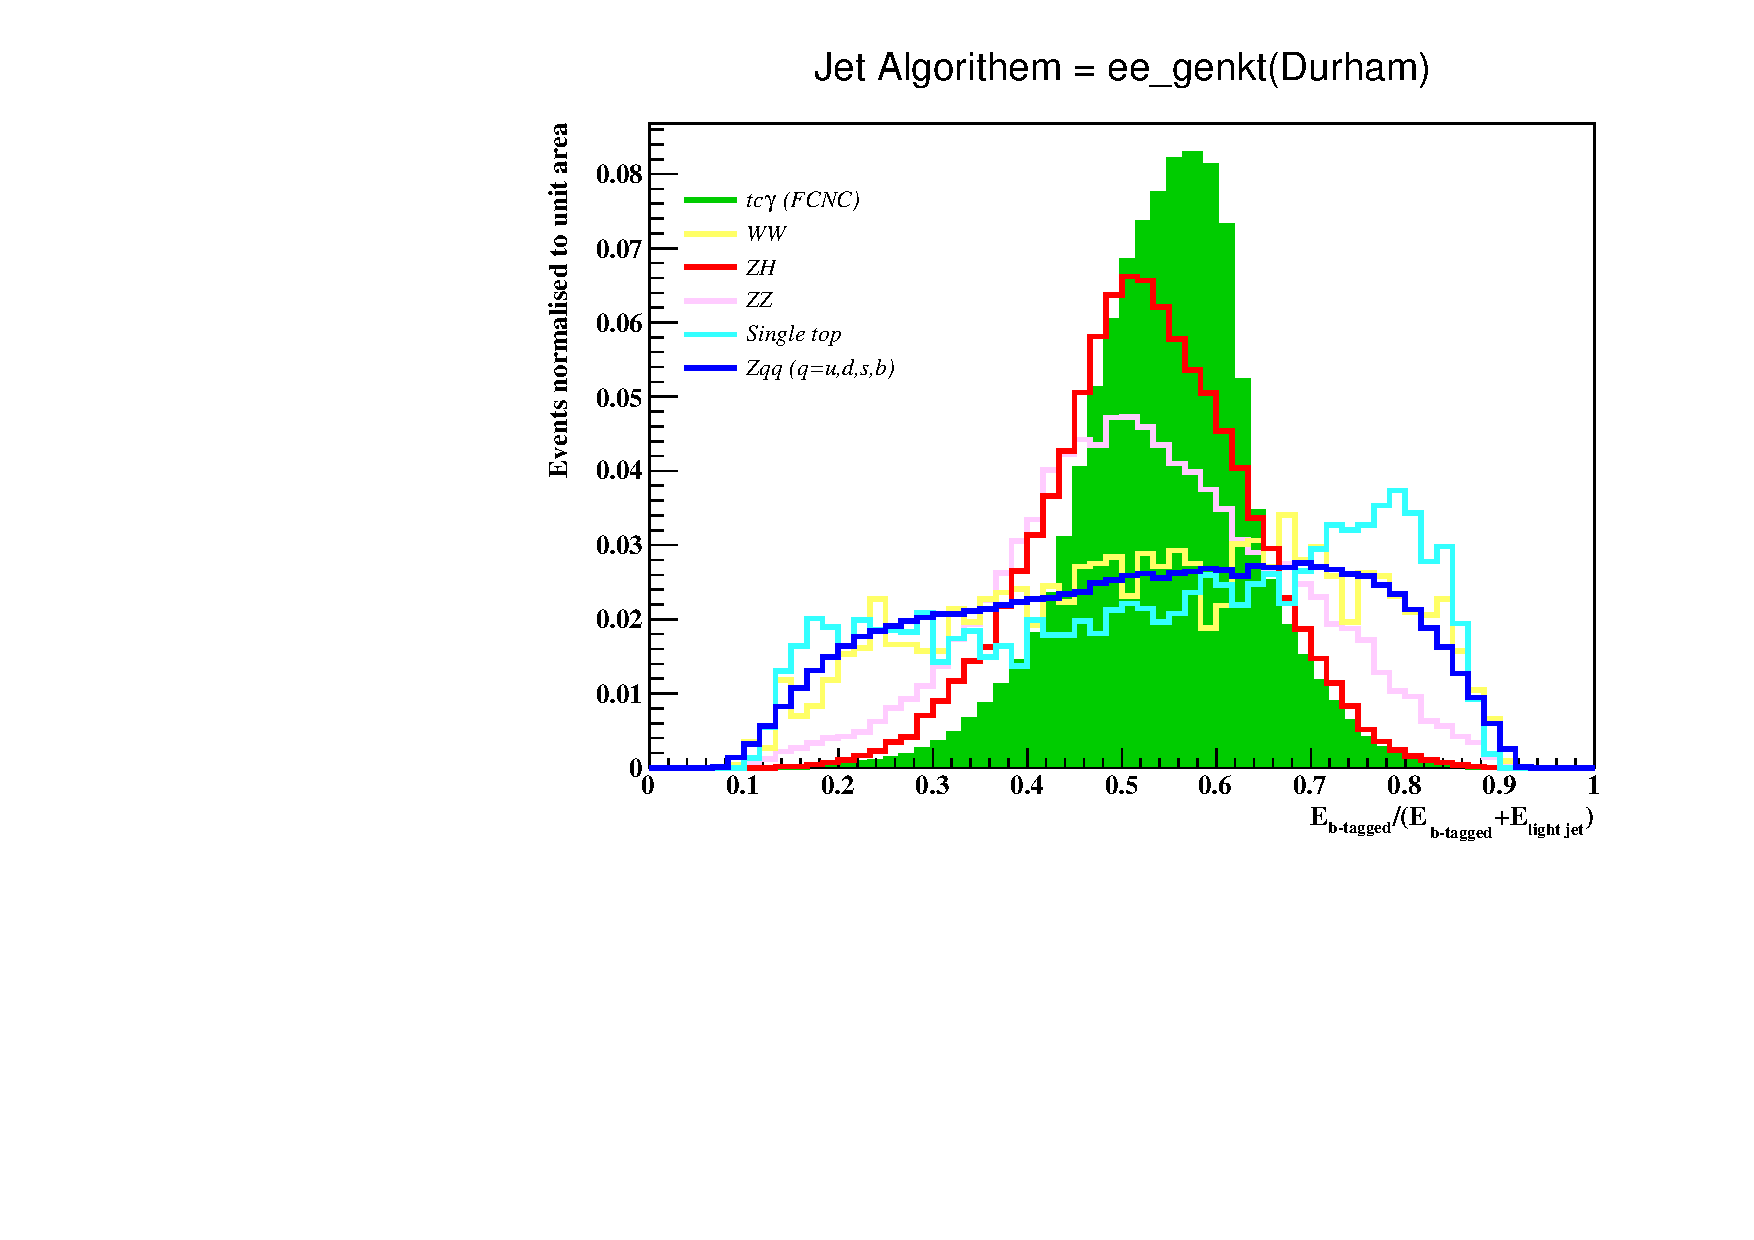
\includegraphics[width=0.40 \textwidth]{Plots-240/Eratio_electron_240.pdf}	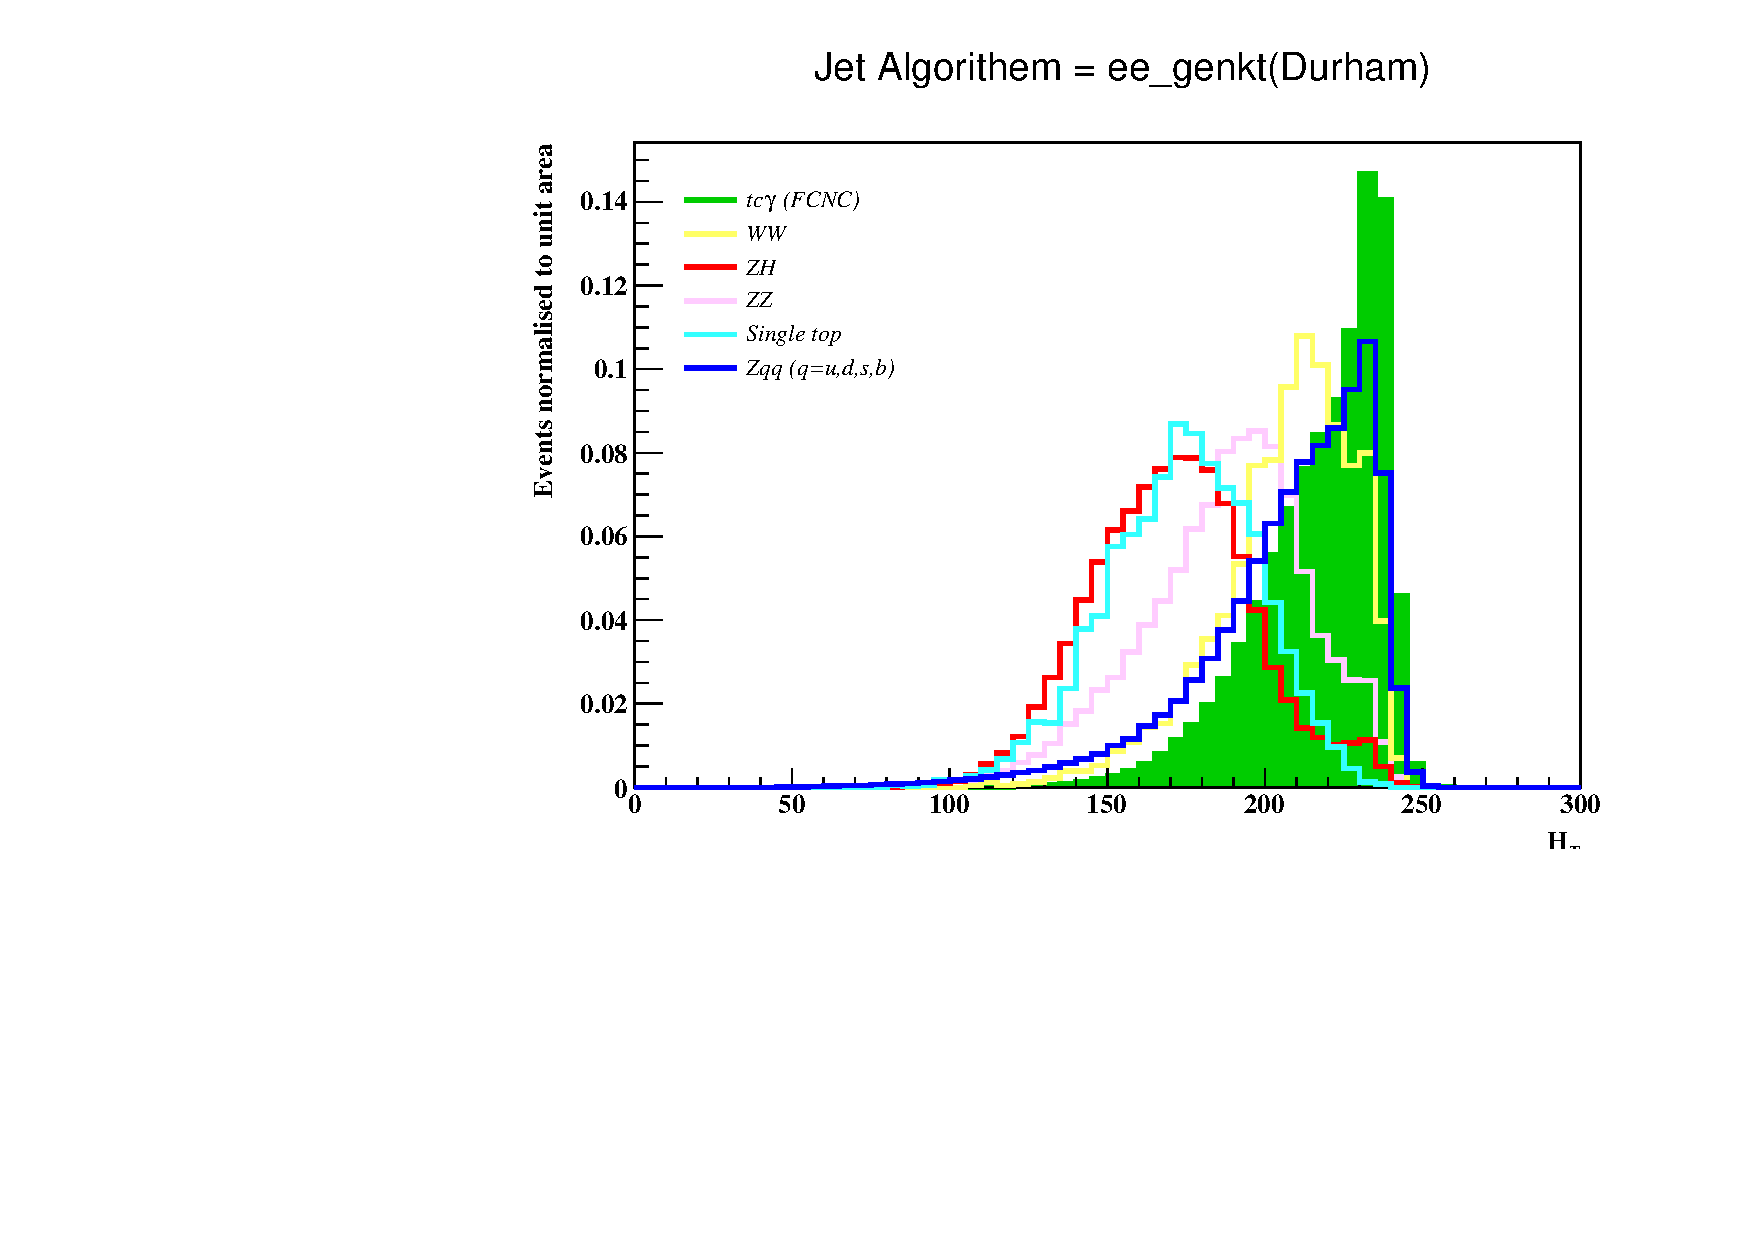
\includegraphics[width=0.40 \textwidth]{Plots-240/Ht_electron_240.pdf}
	\] 
		\[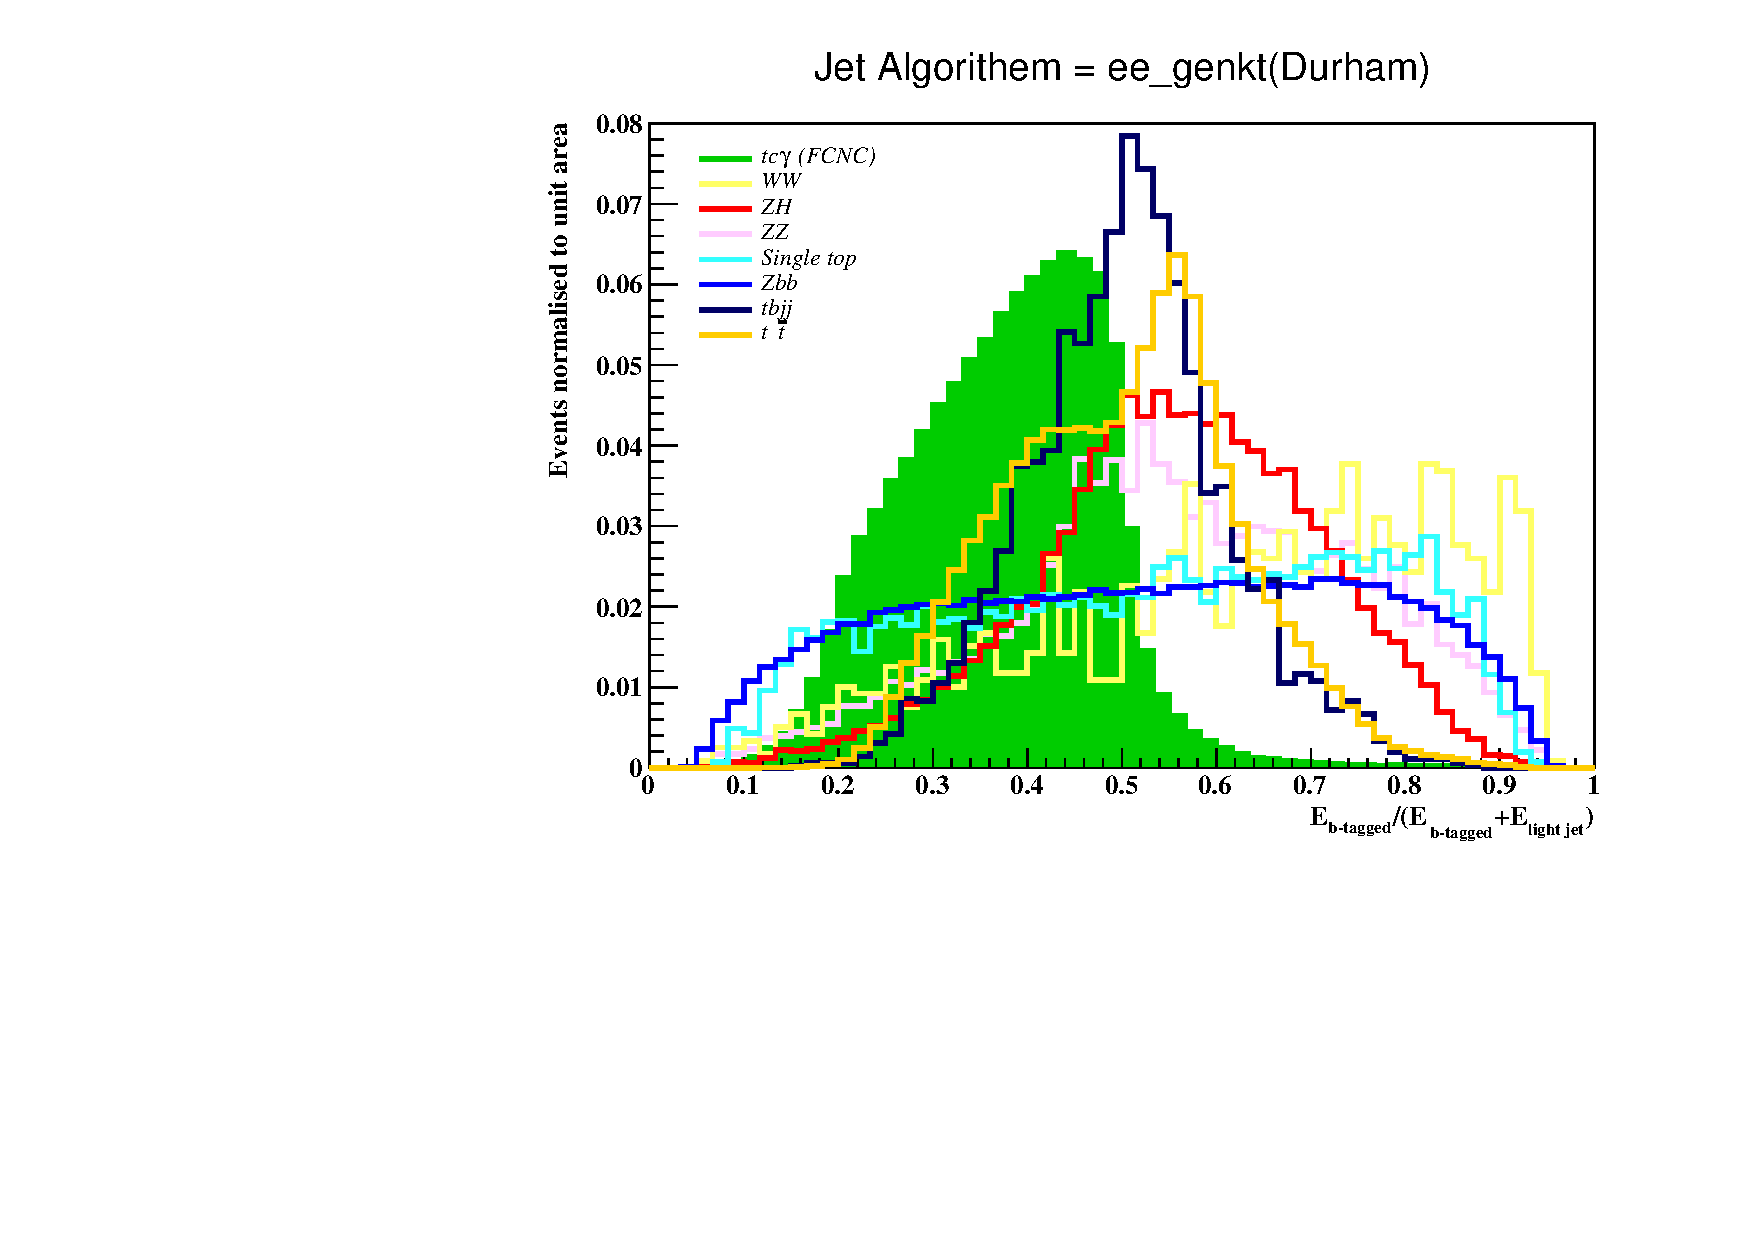
\includegraphics[width=0.40 \textwidth]{Plots-365/Eratio_electron_365.pdf}	
		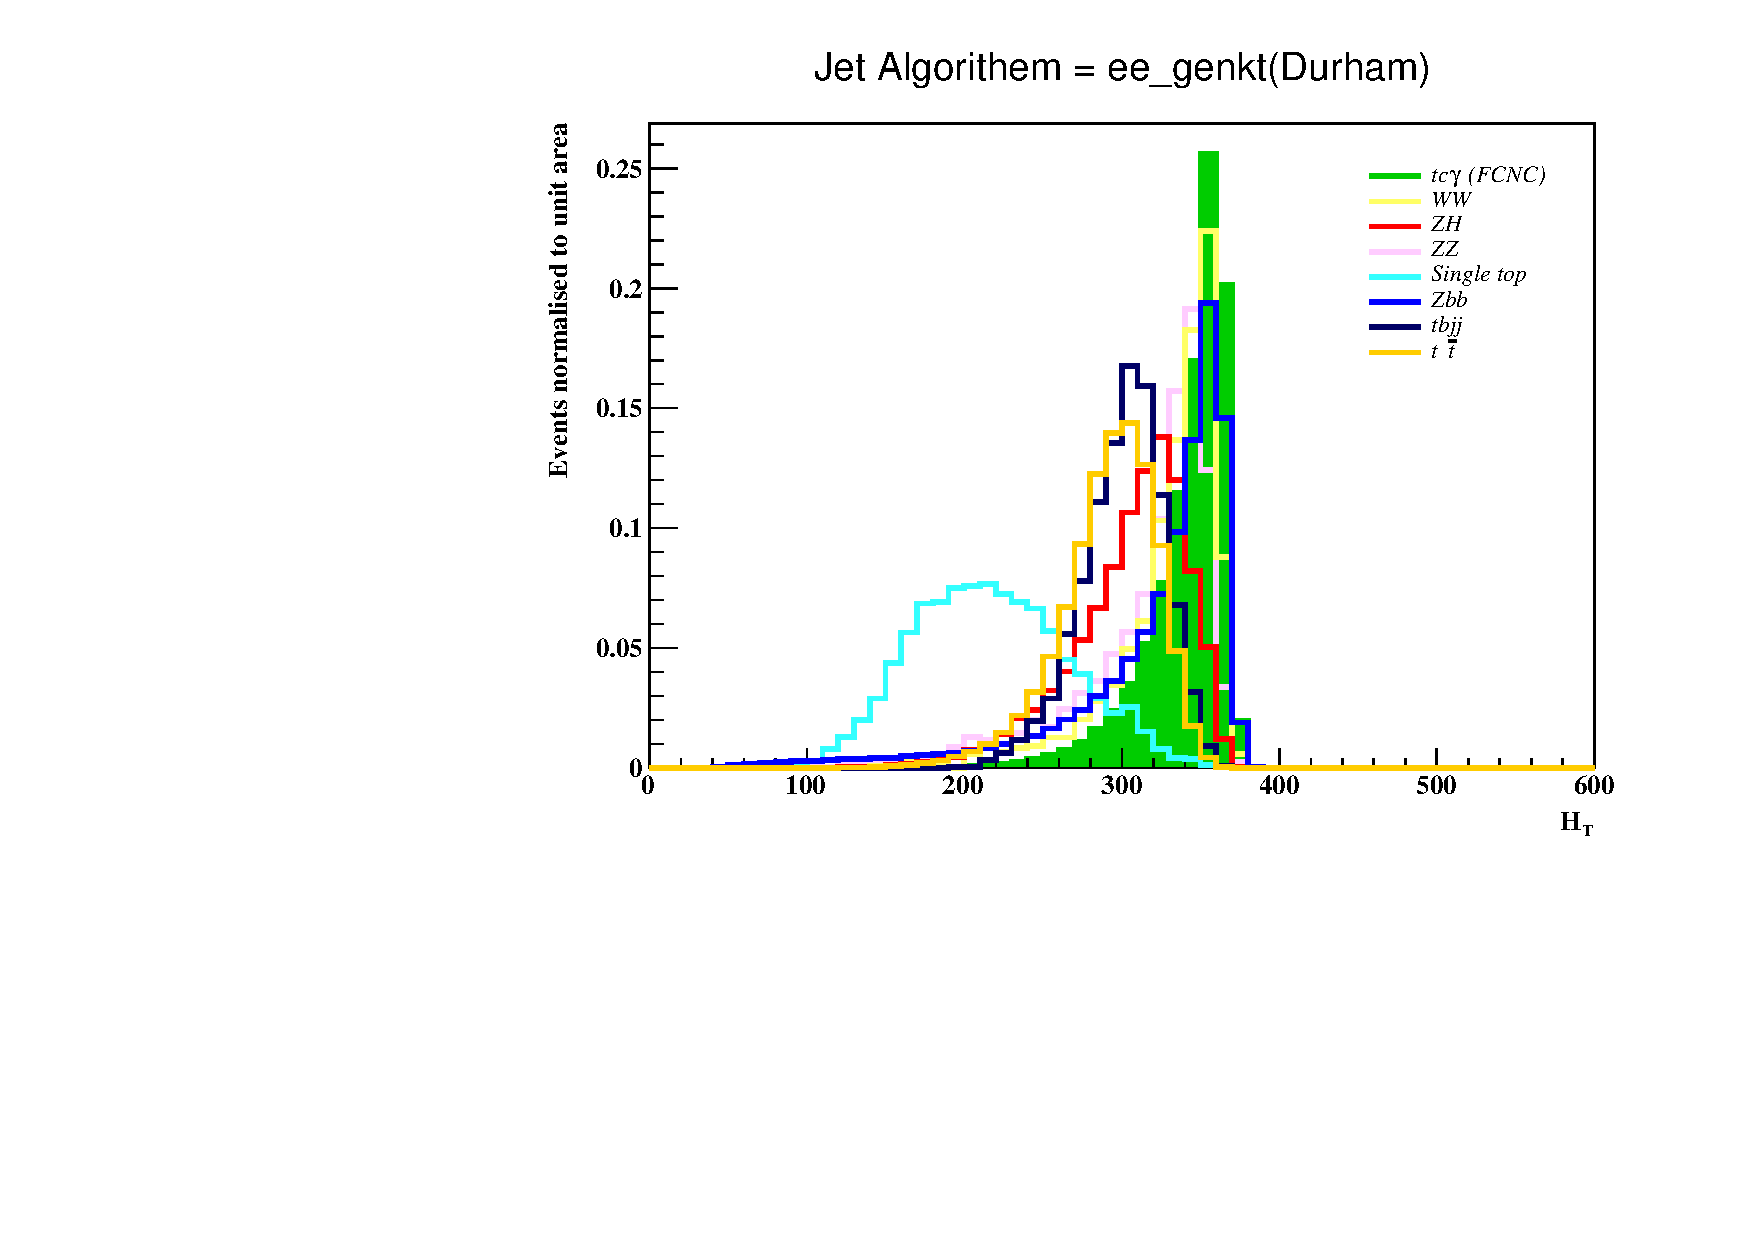
\includegraphics[width=0.4 \textwidth]{Plots-365/Ht_electron_365.pdf}
	\] 
	\end{column}		
\end{columns}
\vspace{0.5cm}
\centering
$H_T$ is scalar sum of  momentum of all outgoing particles.

\end{frame}

%------------------------------------------------
\begin{frame}
	\frametitle{Selection cuts-240 GeV}
	The variables which have the best possible discrimination power between the signal and background processes:
		\begin{columns}[t] % The "c" option specifies centered vertical alignment while the "t" option is 
	%\hspace{-2cm}
	\small
	\begin{column}{0.4\textwidth} % Right column width
            \begin{enumerate}
             
               \item $140$ GeV$ < M_{\rm top} < 190$ GeV.
               \item  $70$ GeV $< M_{\rm W} < 90$ GeV.
               \item  $p_{\rm bjet} > 40$ GeV.
               \item  $p_{\rm lightjet} > 40$ GeV.
               \item $p_{\rm \ell} > 20$ GeV.
               \item  ME $> 30$ GeV.
               \item  $\Delta R (\ell, b_{\rm jet}) < 3.5$.
               \item  $0.35 < E_{\rm bjet}/(E_{\rm bjet}+E_{\rm lightjet}) < 0.7$.
               \item $H_T > 190$ GeV.
             
            \end{enumerate}
            \end{column}
            
            	\begin{column}{0.5\textwidth} % Right column width
            	\vspace{-0.5cm}
            	\[\hspace{1.1cm}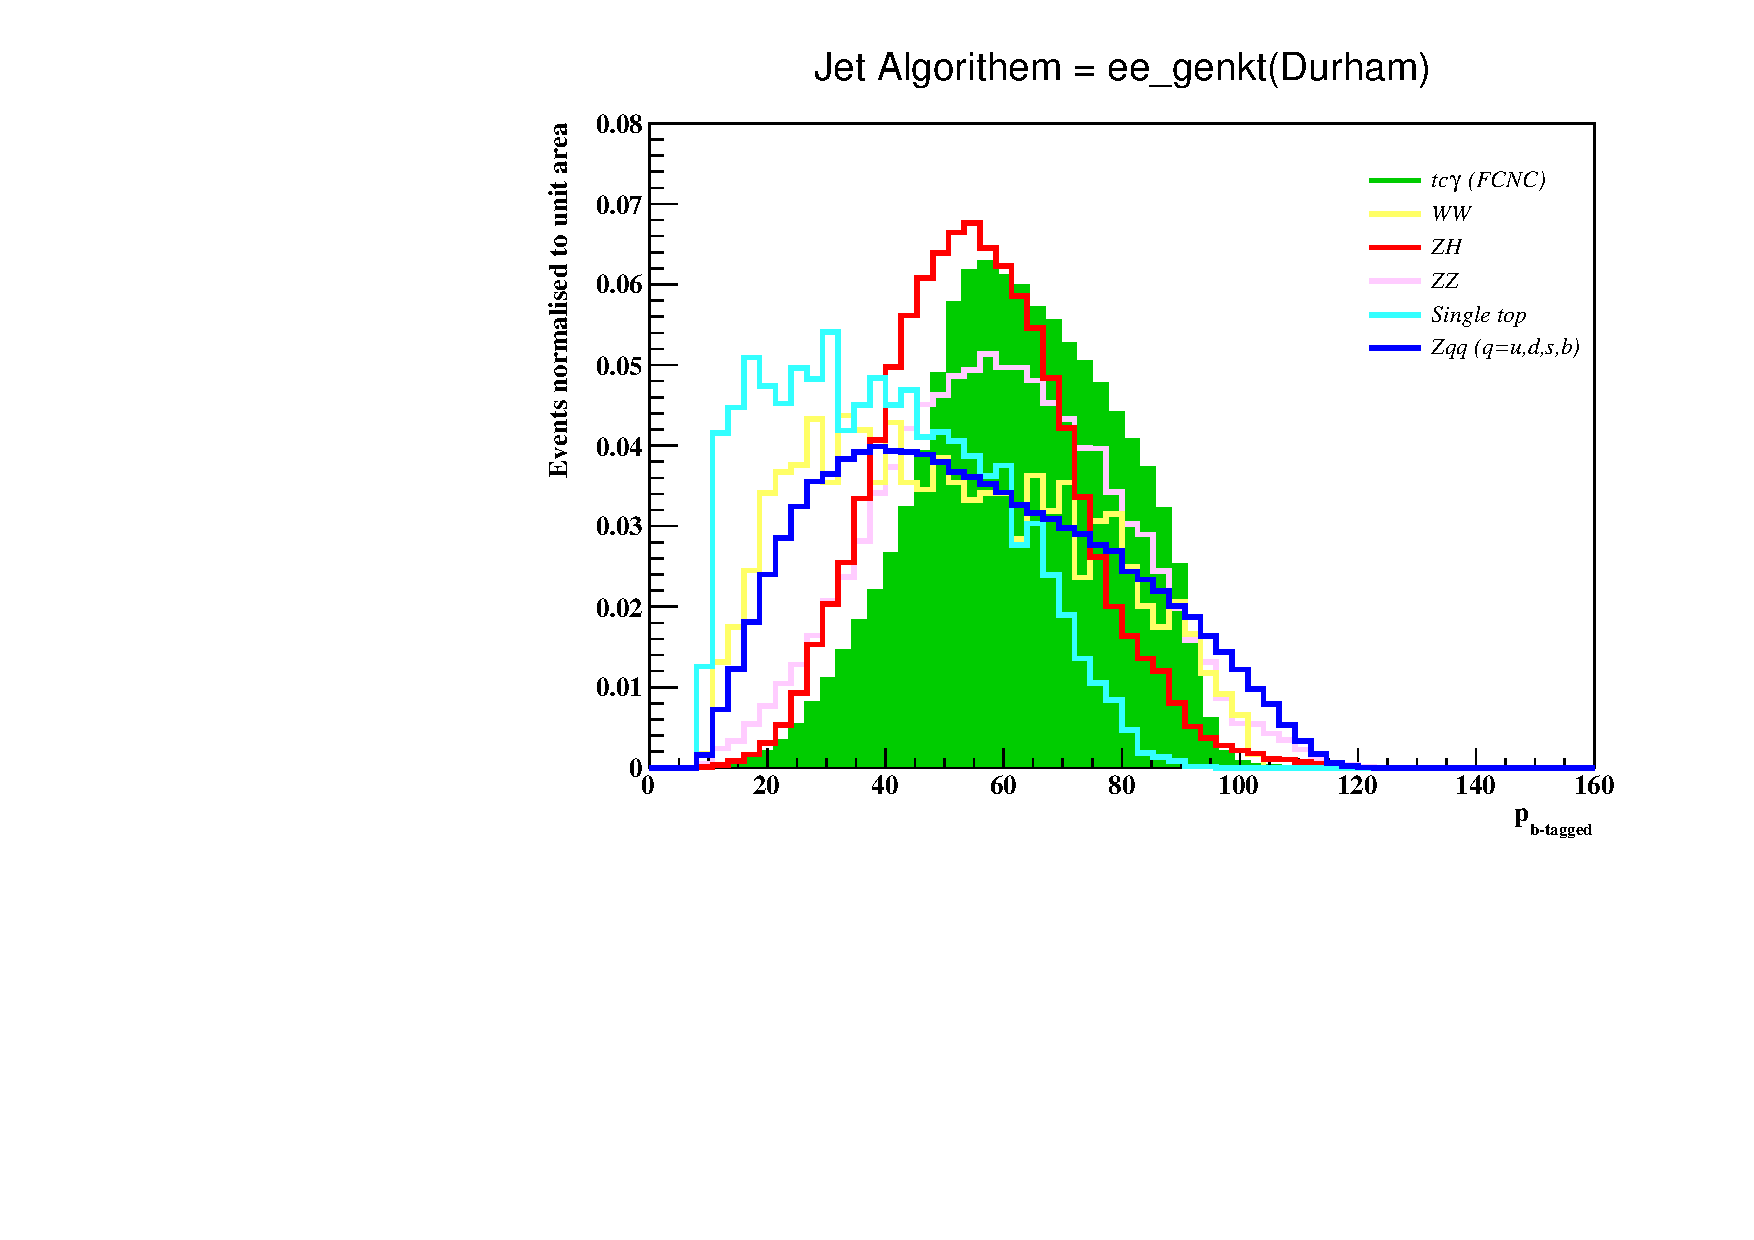
\includegraphics[width=0.55 \textwidth]{Plots-240/pb_electron_240.pdf}\]	\[\hspace{1.1cm}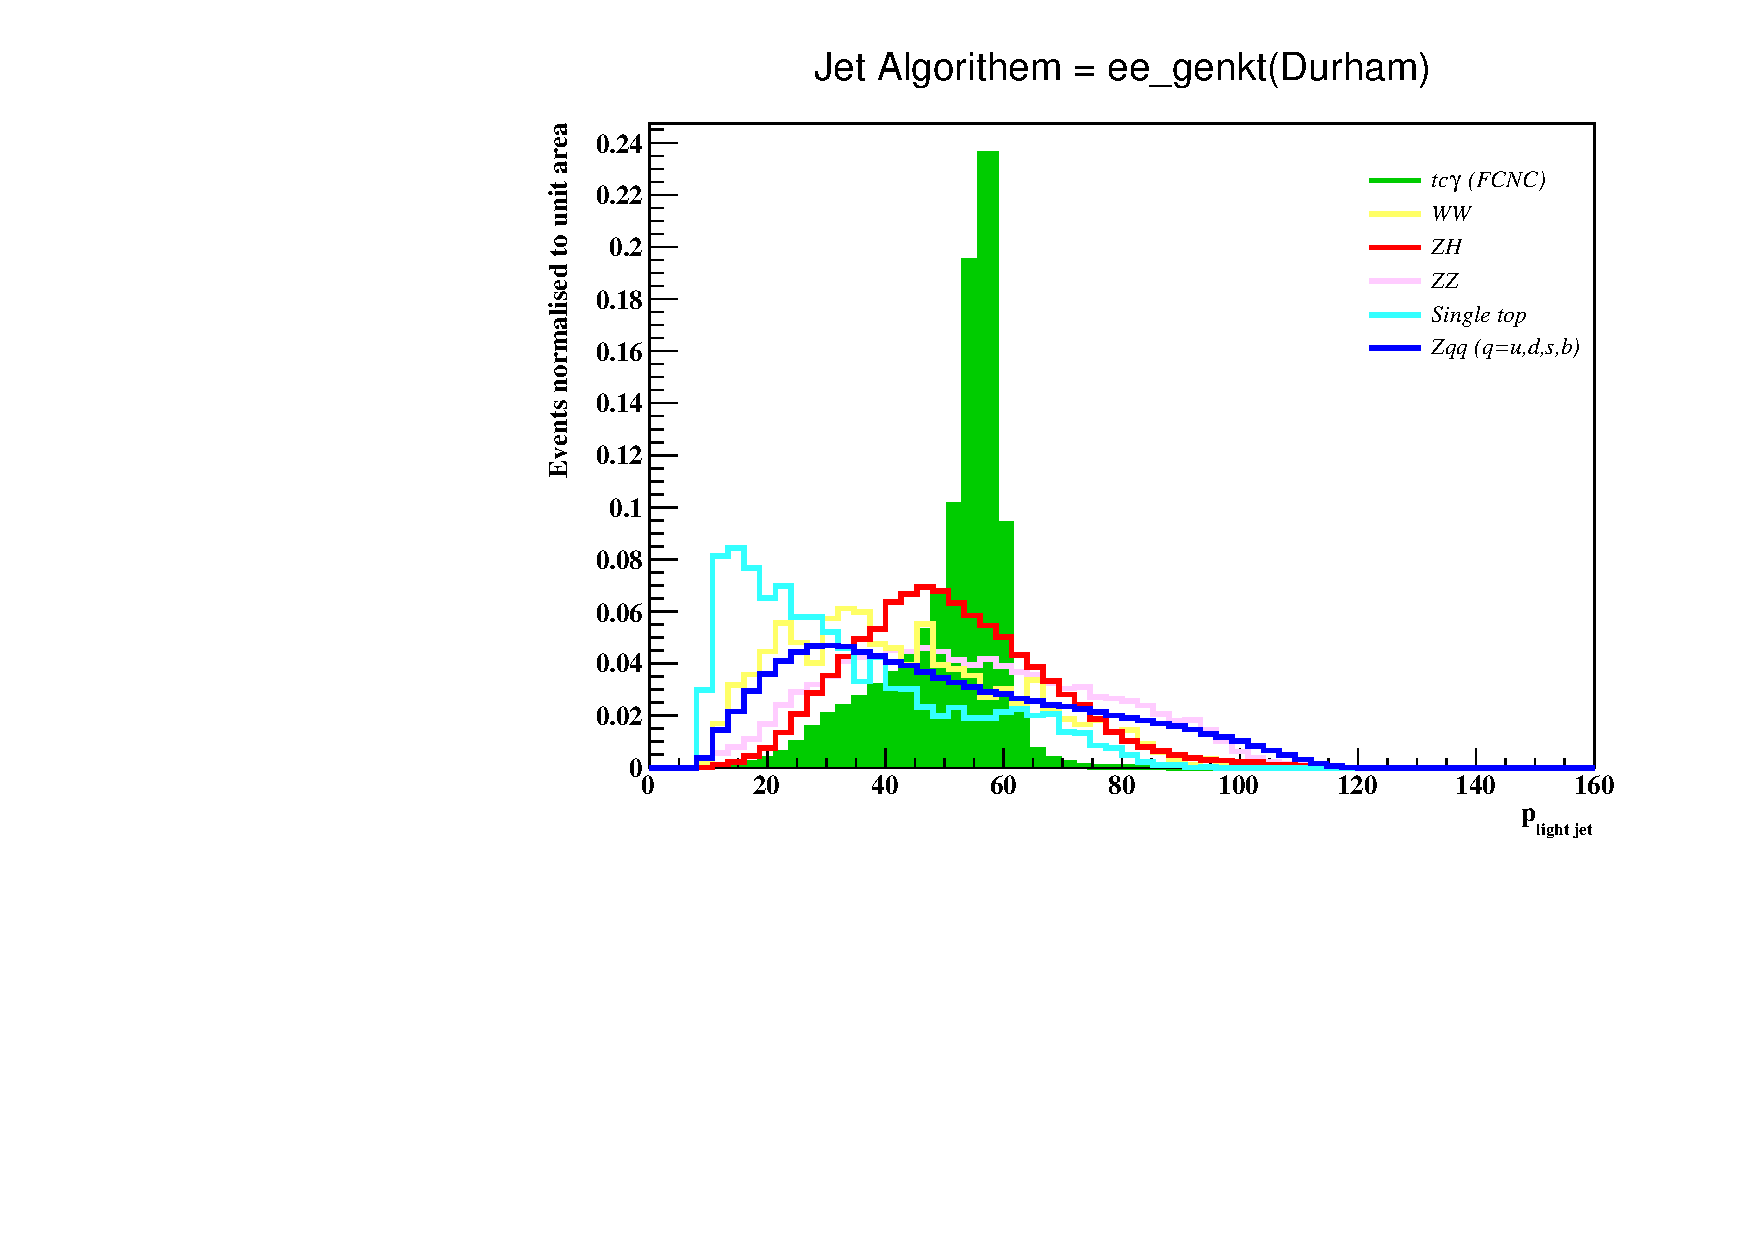
\includegraphics[width=0.55 \textwidth]{Plots-240/pL_electron_240.pdf}
            	\] 
            	 \end{column}
            \end{columns}
            \hspace{-1cm}
            	\[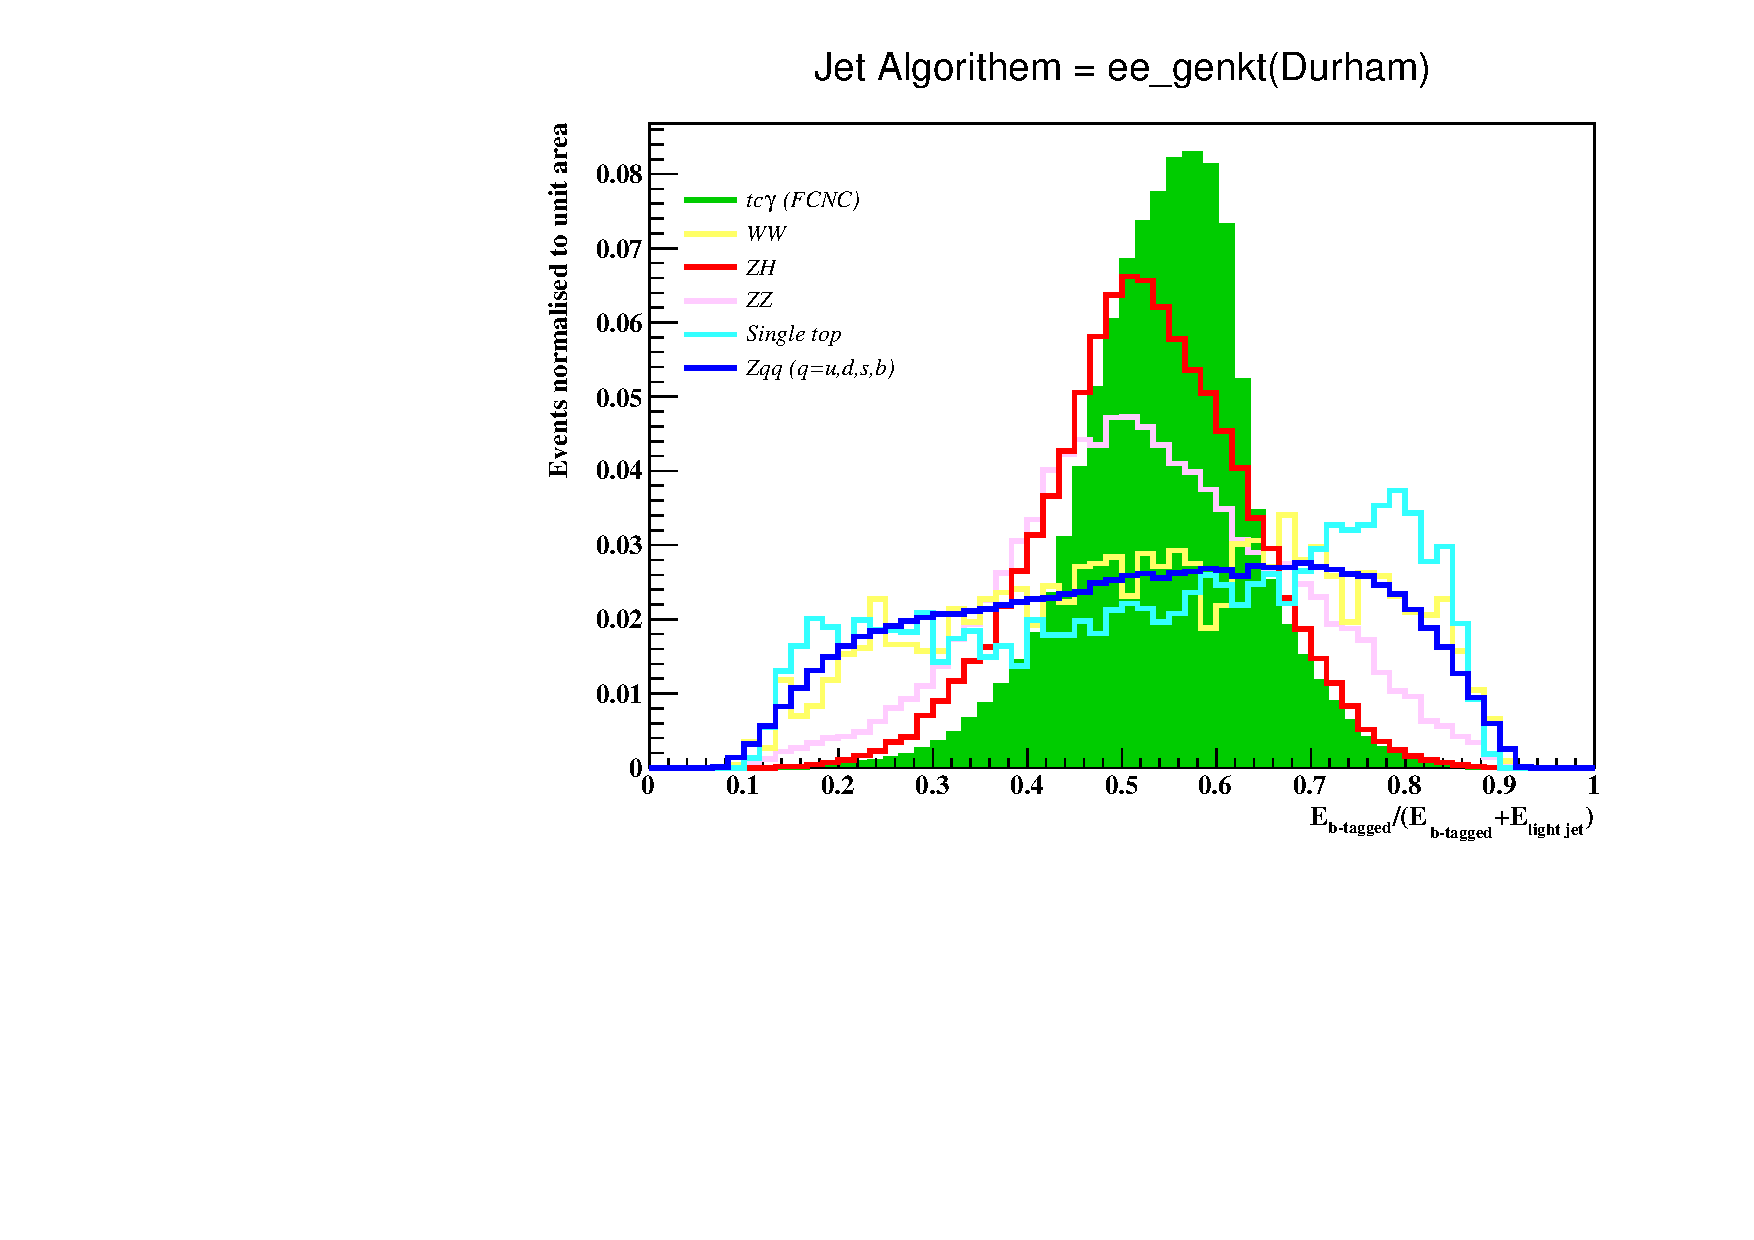
\includegraphics[width=0.28 \textwidth]{Plots-240/Eratio_electron_240.pdf}	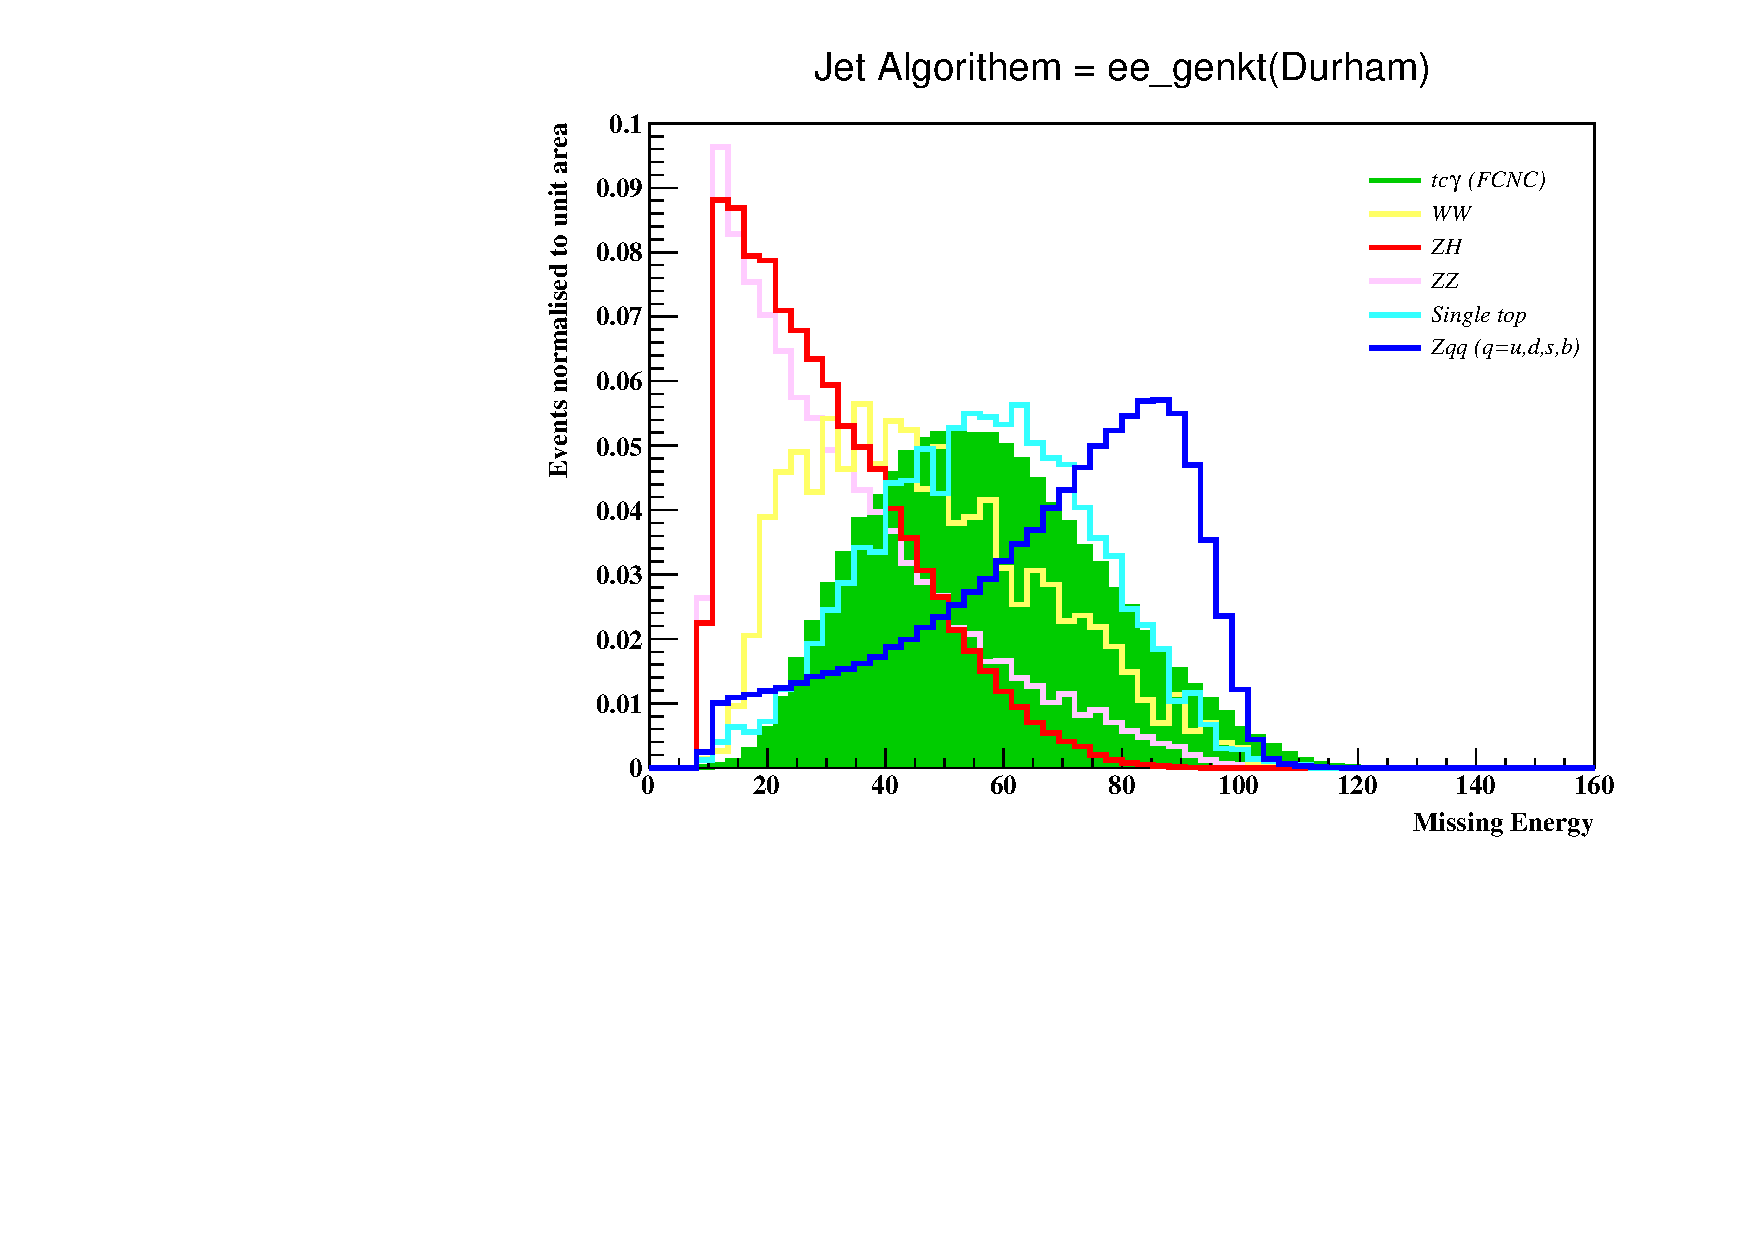
\includegraphics[width=0.28 \textwidth]{Plots-240/met_electron_240.pdf}
            	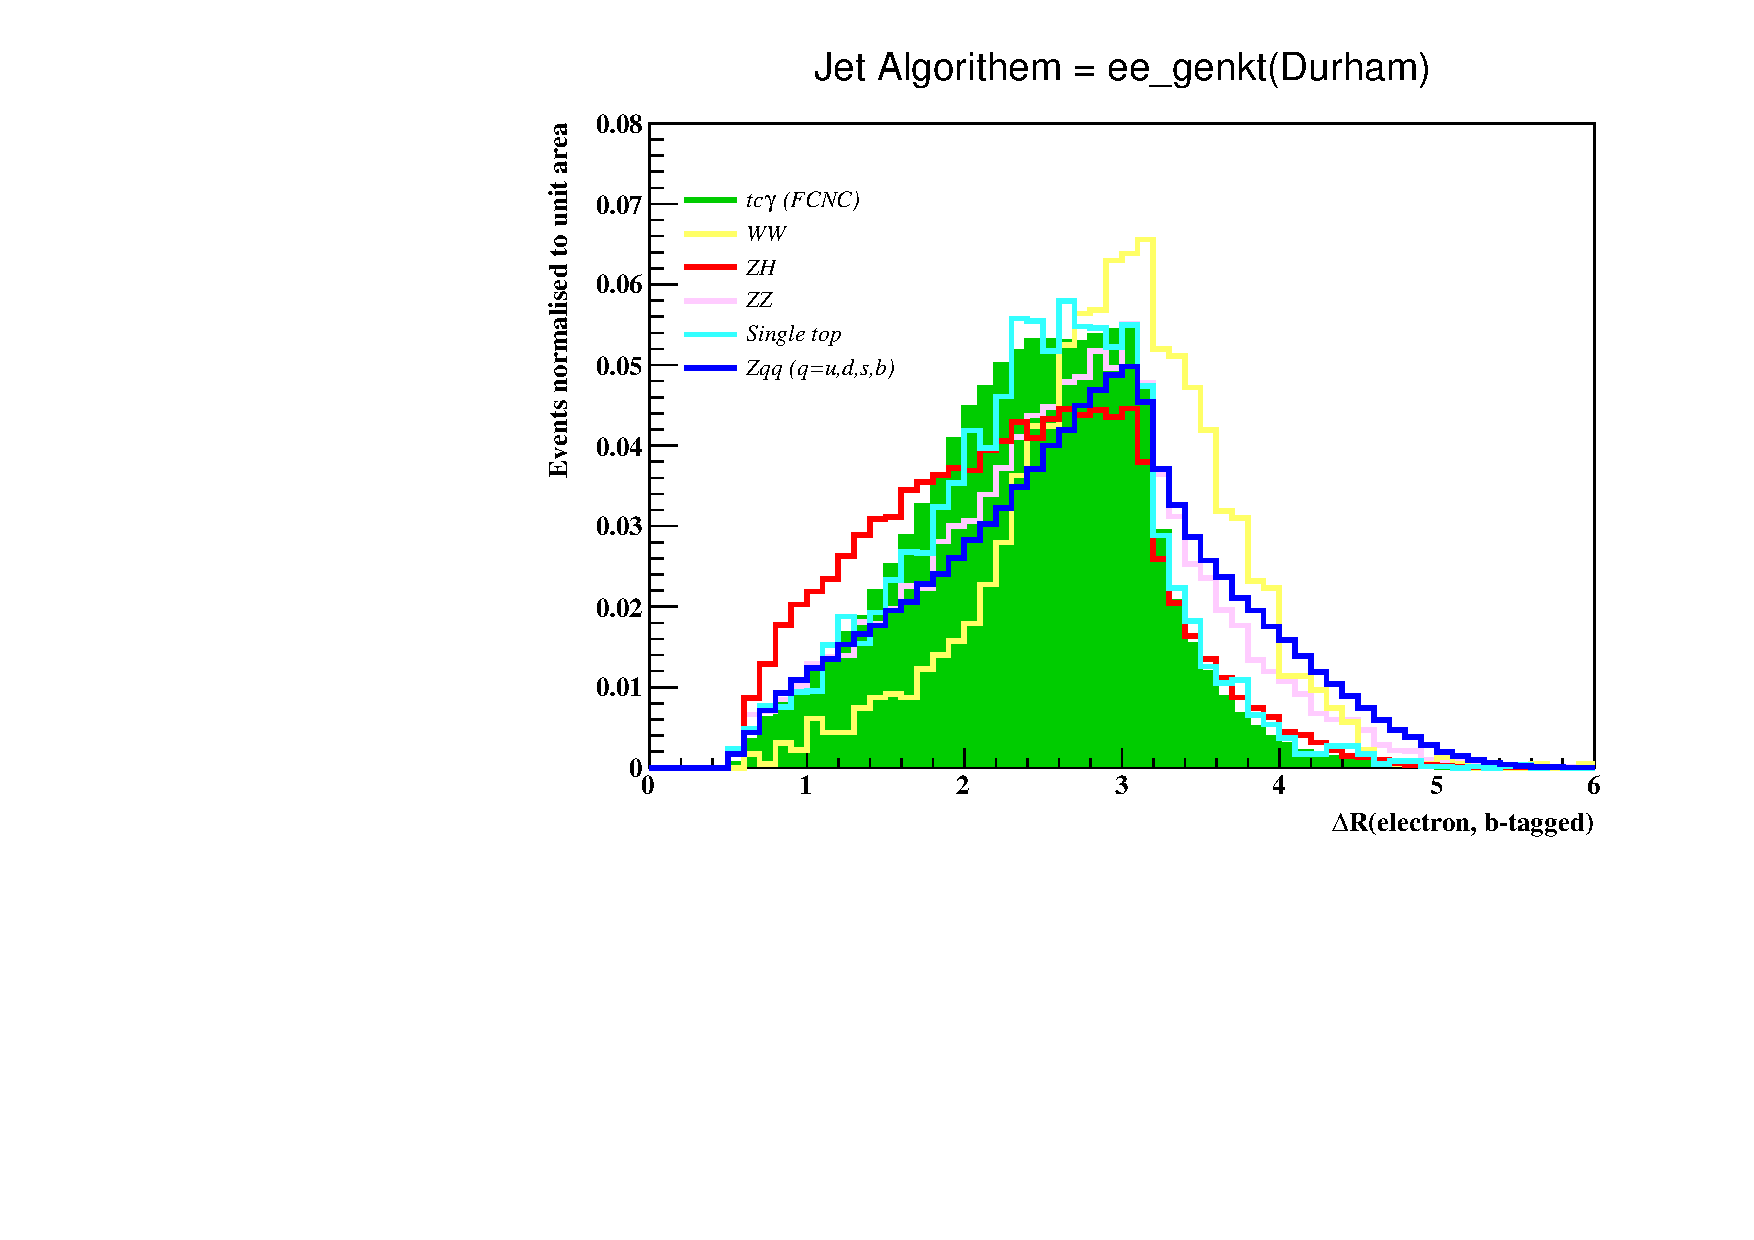
\includegraphics[width=0.28 \textwidth]{Plots-240/Drlbjet_electron_240.pdf}
            \] 
\end{frame}
%------------------------------------------------
\begin{frame}
\frametitle{Selection cuts-365 GeV}

\begin{columns}[t] % The "c" option specifies centered vertical alignment while the "t" option is 
%\hspace{-2cm}


\begin{column}{0.5\textwidth} % Right column width
\vspace{-0.25cm}
\[\hspace{-2.5cm}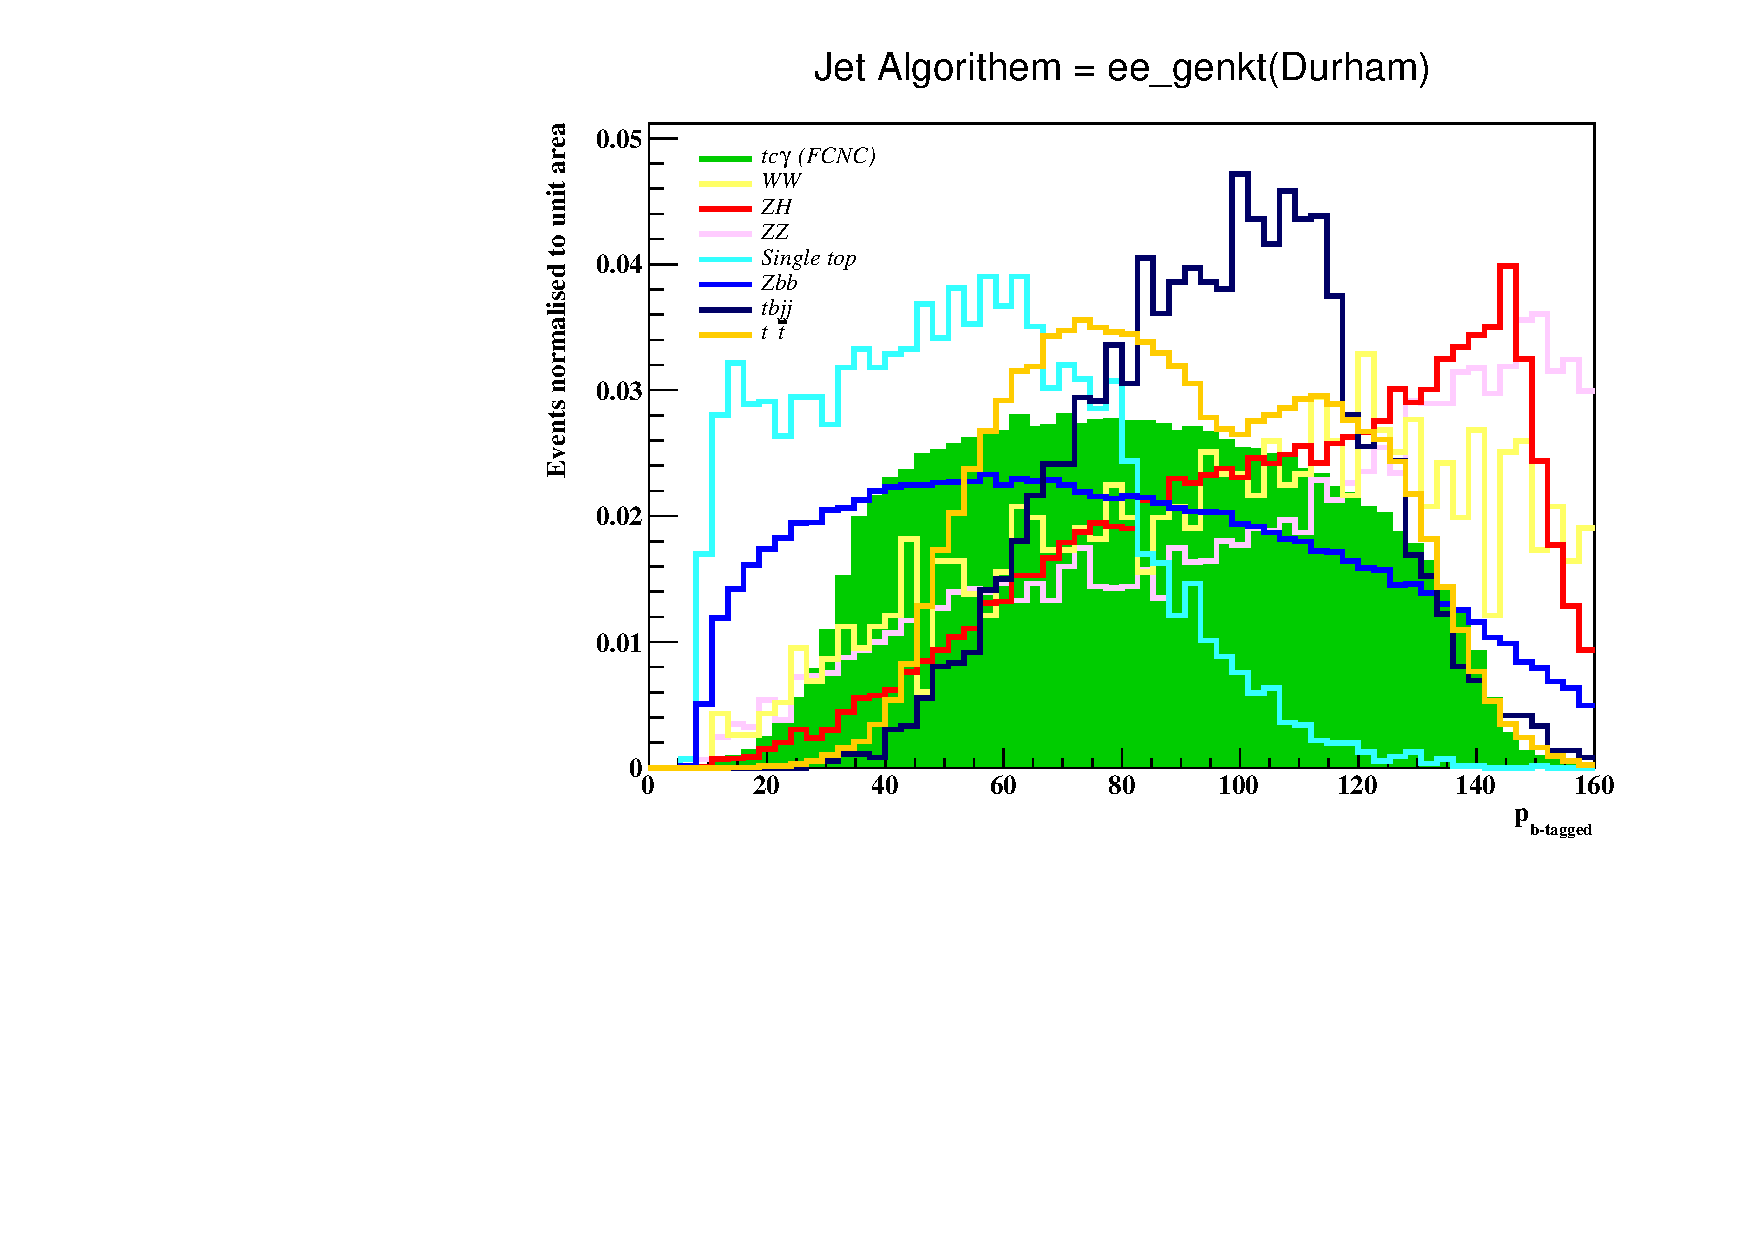
\includegraphics[width=0.53\textwidth]{Plots-365/pb_electron_365.pdf}\]	\[\hspace{-2.5cm}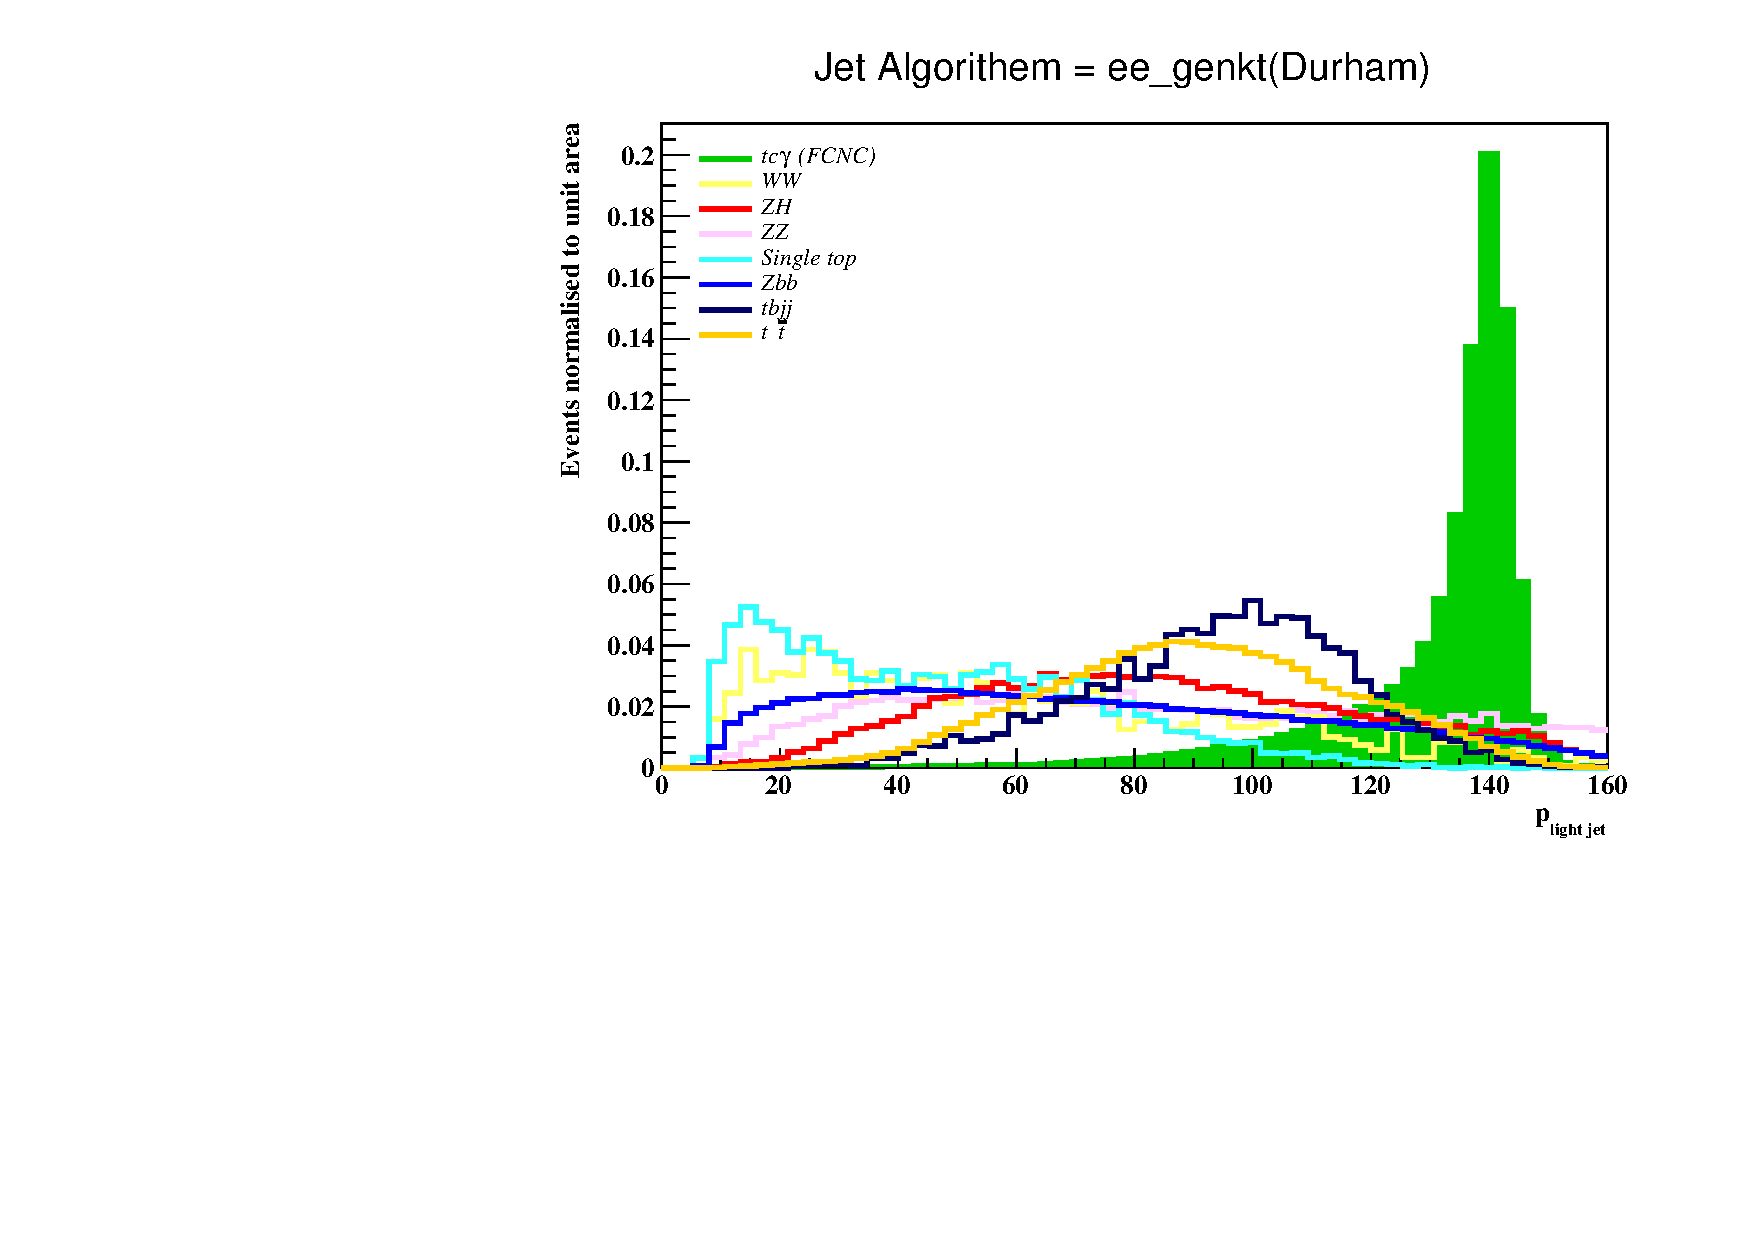
\includegraphics[width=0.53\textwidth]{Plots-365/pL_electron_365.pdf}
\] 
\end{column}
\hspace{-2cm}
\begin{column}{0.5\textwidth} % Right column width
\small
\begin{enumerate}

\item $140$ GeV$ < M_{\rm top} < 190$ GeV.
\item  $70$ GeV $< M_{\rm W} < 90$ GeV.
\item  $p_{\rm bjet} > 30$ GeV.
\item  $p_{\rm lightjet} > 120$ GeV.
\item $p_{\rm \ell} > 20$ GeV.
\item  ME $> 30$ GeV.
\item  $\Delta R (\ell, b_{\rm jet}) < 3.5$.
\item  $0.2 < E_{\rm bjet}/(E_{\rm bjet}+E_{\rm lightjet}) < 0.5$.
\item $H_T > 300$ GeV.

\end{enumerate}
\end{column}
\end{columns}

\[\hspace{-0.5cm}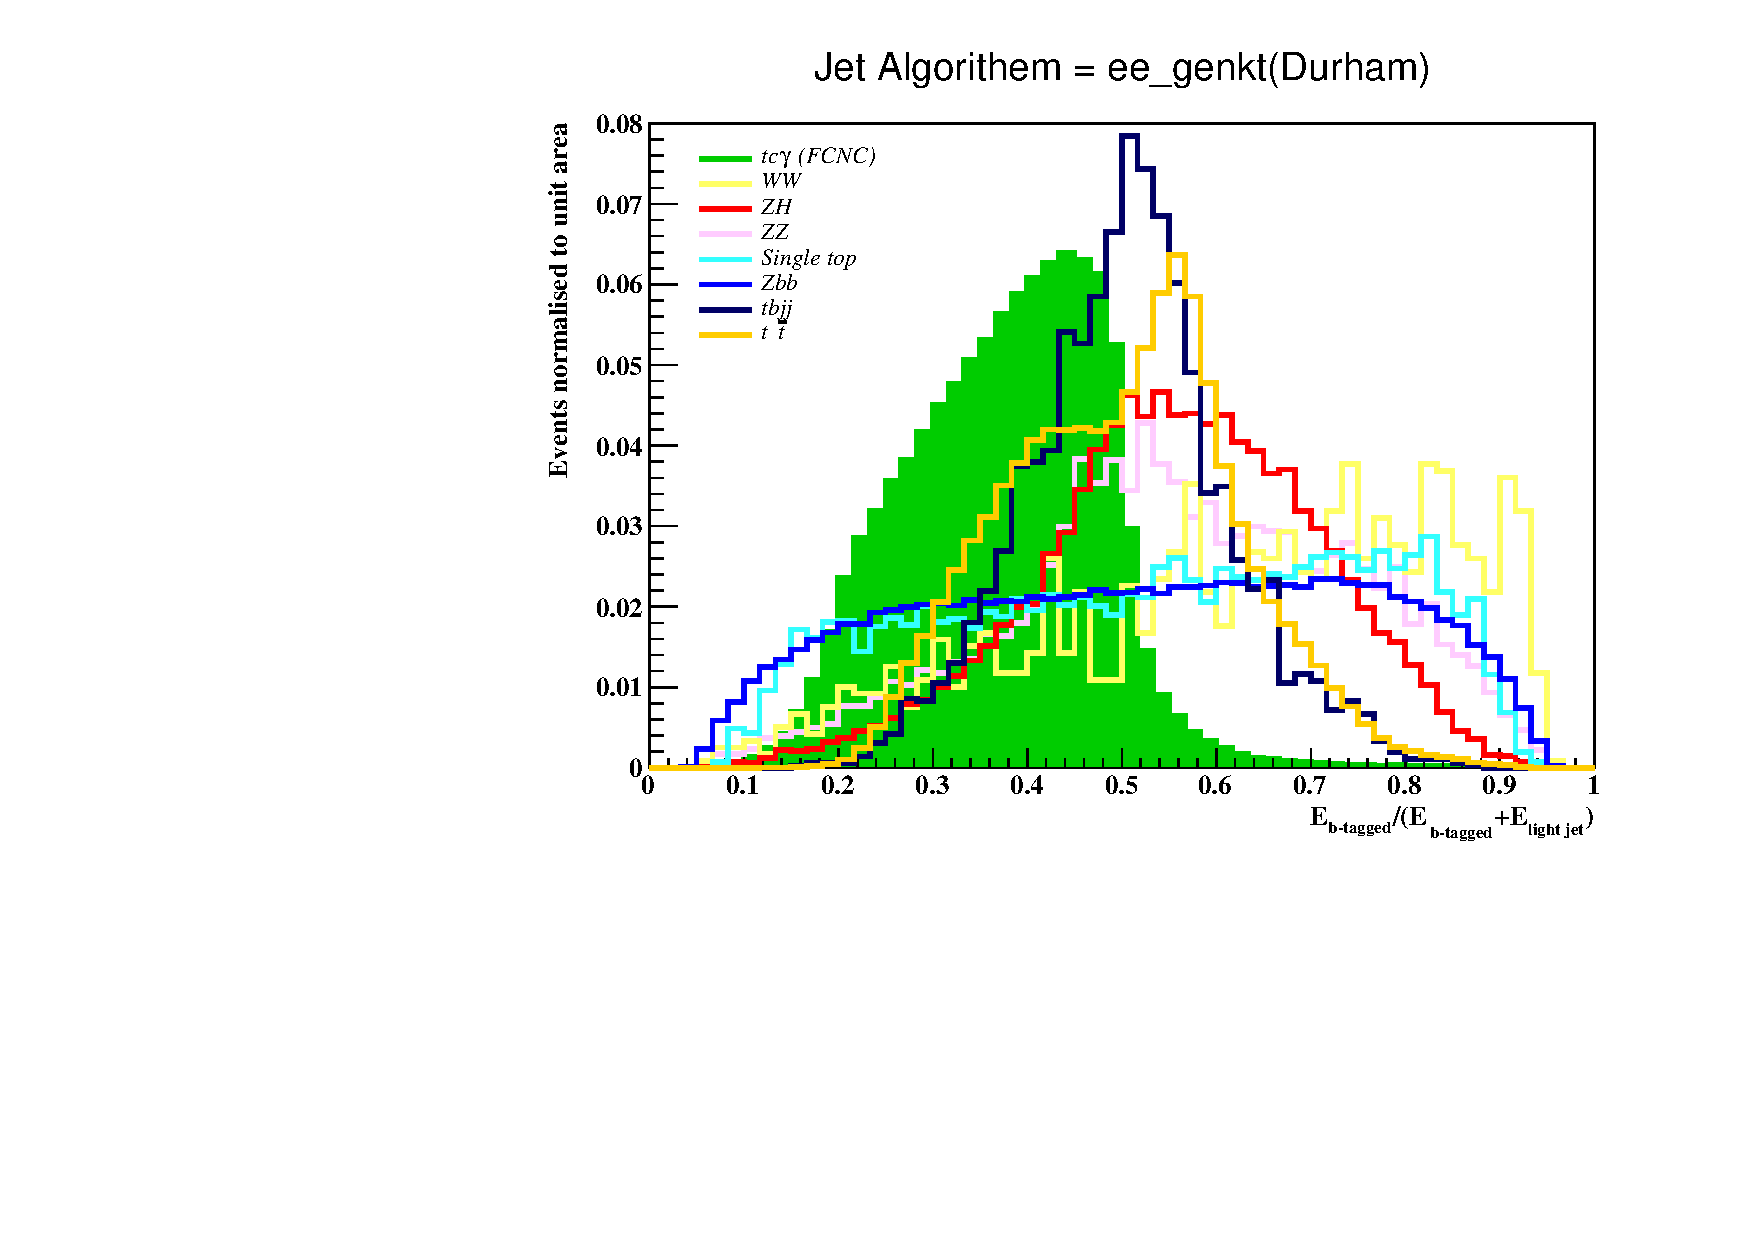
\includegraphics[width=0.28 \textwidth]{Plots-365/Eratio_electron_365.pdf}	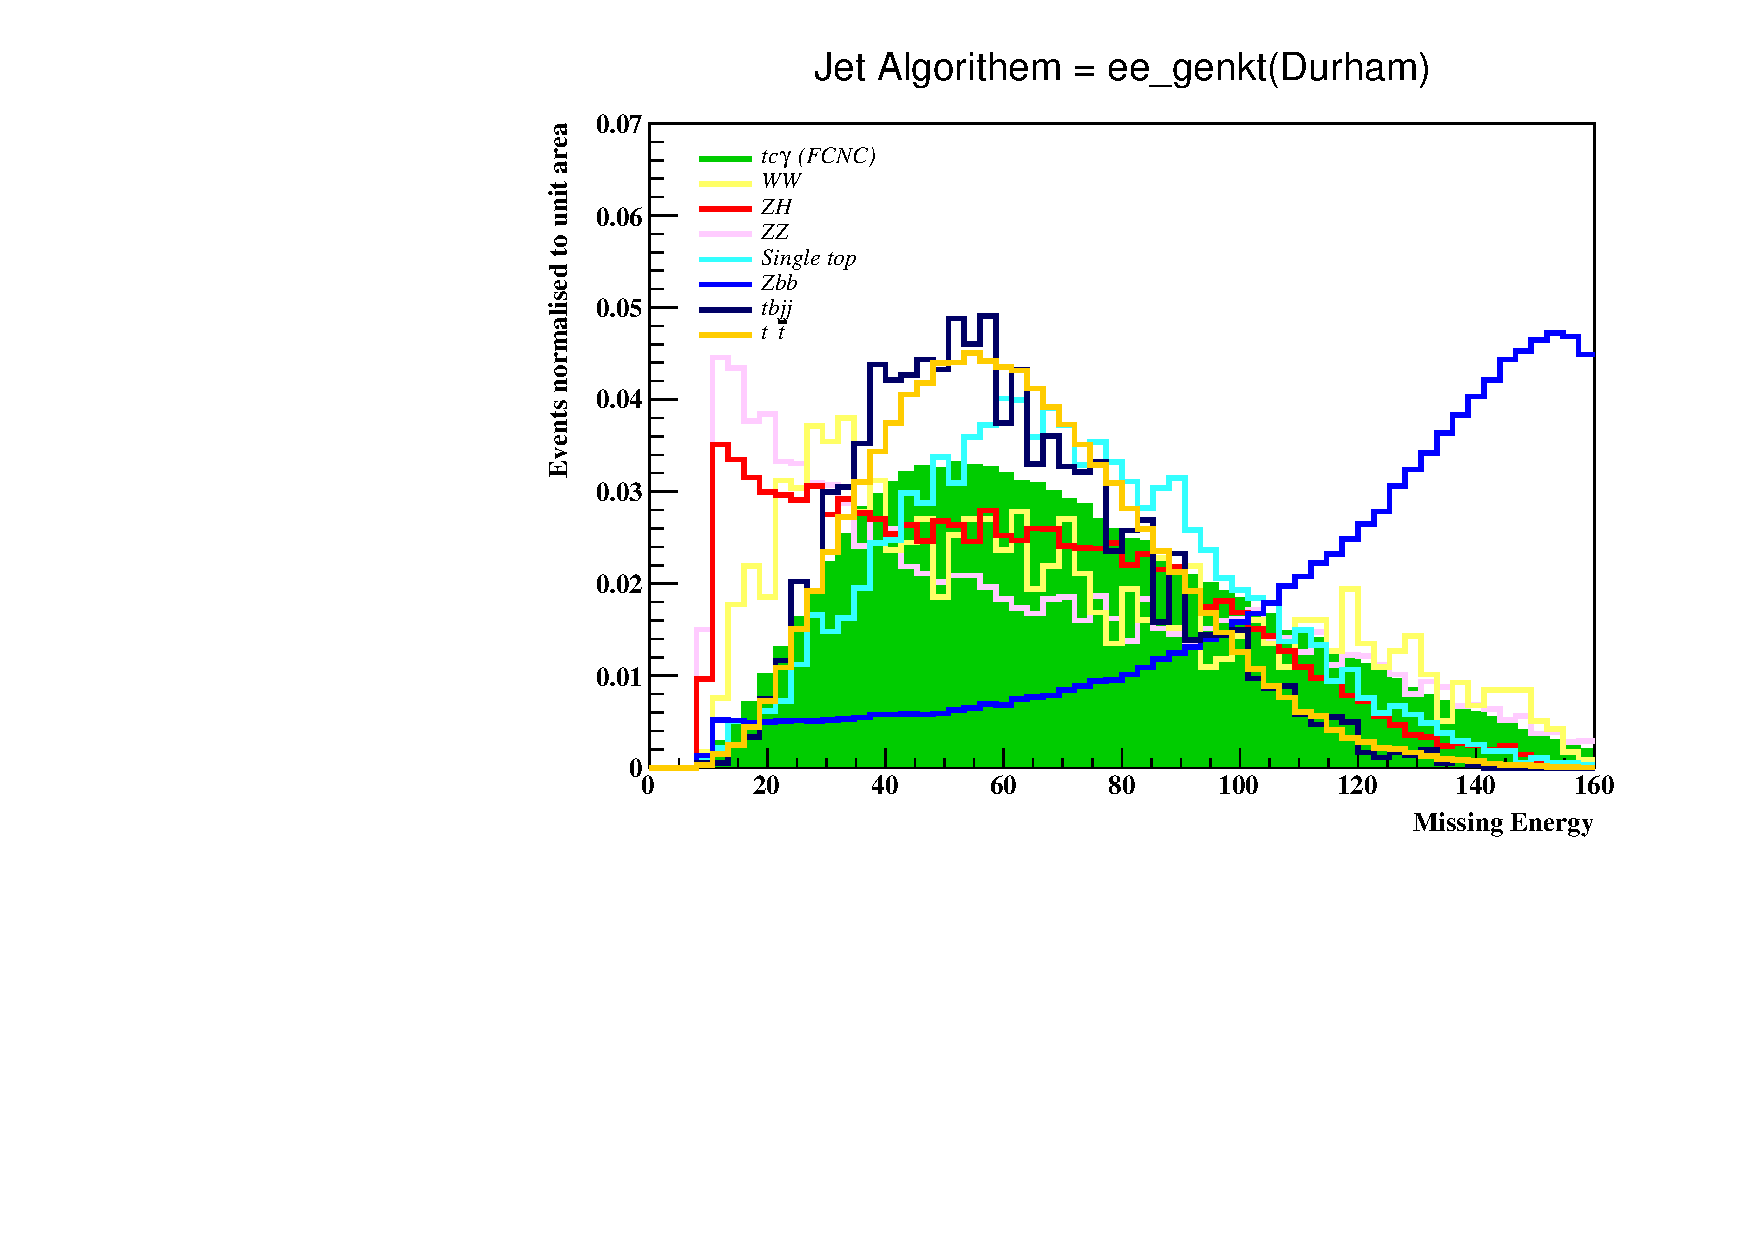
\includegraphics[width=0.28 \textwidth]{Plots-365/met_electron_365.pdf}
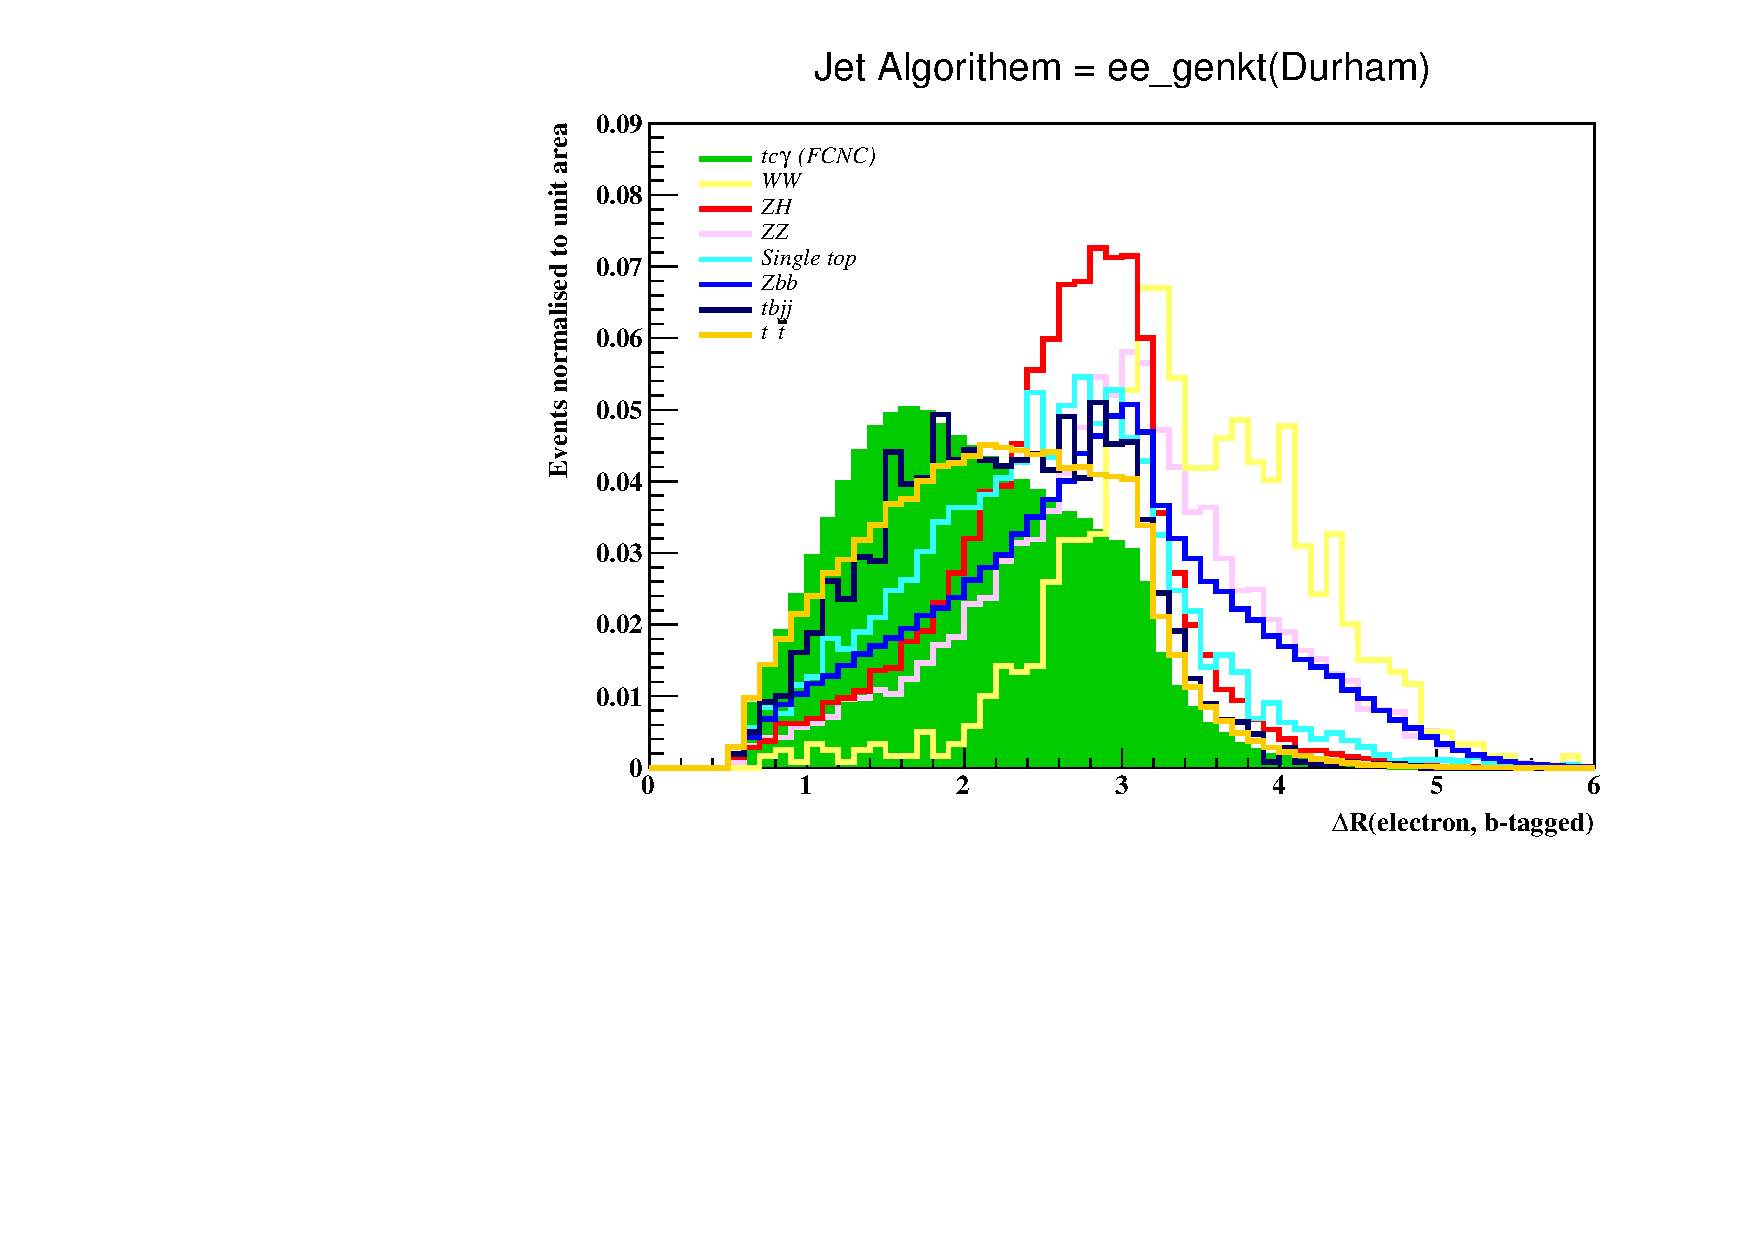
\includegraphics[width=0.28 \textwidth]{Plots-365/Drlbjet_electron_365.pdf}
\] 
\end{frame}

%------------------------------------------------
%\section{Analysis strategy}


\begin{frame}{Cut Flow table}

\begin{tcolorbox}[colback=yellow!5,colframe=yellow!40!black,title=cut flow table for 240 GeV]
\begin{center}
	\resizebox{\linewidth}{!}{%
\begin{tabular}{l|c c c c c c  c c c c c  }  \hline
$\sqrt {s}$ = 240 GeV   ~&~ $tc\gamma$  ~&~ $tcZ$   ~&  ~  ZH     ~&  ~ WW  &  ~  ZZ ~ &~ eebb ~&~ eeqq (q=uds) ~&~ single top  \\  \hline
Cross section    ~&~  $14.327$  ~&~ $34.132$  ~&~    $201.868$        ~&~  $16438.5$   ~&~    $1358.99$  ~&~  $455.7$ ~&~  $1635.9$  ~&~  $0.010753$       \\ 
Preselection    ~&~  $3.1542$  & $7.5154$  &    $1.1953$        &  $3.75948$   &    $2.76677$  &  $19.251$ &  $0.155146$  &  $0.0003208$        \\ 
Final selection
&  $1.3686$  & $3.2622$  &    $0.00847$        &  $0.254797$   &    $0.01127$  &  $0.1807$ &  $0.001439$  &  $3.2259\times10^{-7}$       \\   \hline  \hline
\end{tabular}
}
\end{center}
\end{tcolorbox}


\begin{center}
\begin{tcolorbox}[colback=yellow!5,colframe=yellow!40!black,title=cut flow table for 365 GeV]
	\resizebox{\linewidth}{!}{%
\begin{tabular}{l|c c c c  c c  c c c c c  }  \hline
$\sqrt {s}$ = 365 GeV      ~&~ $tc\gamma$  ~&~ $tcZ$   ~&~ ZH   ~&~  WW  ~&~ ZZ ~&~ $t \bar{t}$                      ~&~ eebb ~&~ single top ~&~ single top ($tbjj$)  \\  \hline
Cross section    ~&~  $25.958$  ~&~  $50.9517$    ~&~  $117.3$ ~&~    $10716.5$     ~&~  $642.8$  ~&~ $800.0$        ~&~  $615.2$  ~&~  $0.227$  ~&~ $5.98$       \\ 
Preselection    ~&~  $5.2107$  ~&~  $10.2299$    ~&~  $0.6240$ ~&~  $2.55696$     ~&~  $1.21039$  ~&~ $39.7574$    ~&~  $25.0175$  ~&~  $0.006297$  ~&~ $0.2159$       \\ 
Final selection    ~&~  $1.9599$  ~&~  $4.3406$    ~&~  $0.00410$ ~&~ $0.00857$  ~&~  $0.00809$  ~&~ $1.10752$  ~&~  $0.004332$  ~&~ $2.276\times 10^{-6}$  ~&~ $0.006947$       \\  \hline  \hline
\end{tabular}

}
\end{tcolorbox}
\end{center}
\end{frame}
%------------------------------------------------
\section{Results}
\small
\begin{frame}
	\frametitle{Results}
	 $ 95\%$ CL upper limts on the anomalous FCNC couplings and consequently on the branching ratios are estimated by using Higgs Combine tools.
 \begin{block}{\centering\begin{tabularx}{\dimexpr\textwidth-2\tabcolsep}{@{}p{0.56\textwidth}@{}X@{}X@{}}%
\textcolor{white}{$\sqrt{s}=240$ GeV $\&  \mathcal{L}=5$ ab$^{-1}$}	& \textcolor{white}{$Br (t \to c \gamma )$} & \textcolor{white}{$Br (t \to c Z)$}\end{tabularx}}%
\centering
\rowcolors{1}{RowColorOdd}{RowColorEven}%
\begin{tabularx}{\dimexpr\textwidth-2\tabcolsep}{@{}p{0.56\textwidth}@{}X@{}X@{}}
Electron channel       &  ~  $9.60 \times 10^{-5}$        & ~ $3.53 \times 10^{-5}$       \\    
Muon channel           &  ~  $6.29 \times 10^{-5}$        & ~ $2.31 \times 10^{-5}$      
\end{tabularx}%
\end{block}%

\begin{block}{\centering\begin{tabularx}{\dimexpr\textwidth-2\tabcolsep}{@{}p{0.56\textwidth}@{}X@{}X@{}}%
	\textcolor{white}{$\sqrt{s}=365$ GeV  $\&\mathcal{L}=1.5$ ab$^{-1}$}	& \textcolor{white}{$Br (t \to c \gamma )$} & \textcolor{white}{$Br (t \to c Z)$}\end{tabularx}}%
\centering
\rowcolors{1}{RowColorOdd}{RowColorEven}%
\begin{tabularx}{\dimexpr\textwidth-2\tabcolsep}{@{}p{0.56\textwidth}@{}X@{}X@{}}
Electron channel       &  ~  $1.65 \times 10^{-4}$        & ~ $6.96 \times 10^{-5}$       \\    
Muon channel           &  ~  $1.47 \times 10^{-4}$        & ~ $6.19 \times 10^{-5}$          
\end{tabularx}%
\end{block}%

\setbeamercolor{block title}{use=structure,fg=white,bg=purple!75!black}
\setbeamercolor{block body}{use=structure,fg=black,bg=white!20!white}
\begin{block}{\centering\begin{tabularx}{\dimexpr\textwidth-2\tabcolsep}{@{}p{0.56\textwidth}@{}X@{}X@{}}%
	\textcolor{white}{}	& \textcolor{white}{$Br (t \to c \gamma )$} & \textcolor{white}{$Br (t \to c Z)$}\end{tabularx}}%
\centering
\rowcolors{1}{RowColorOdd}{RowColorEven}%
\begin{tabularx}{\dimexpr\textwidth-2\tabcolsep}{@{}p{0.56\textwidth}@{}X@{}X@{}}
    Energy $\&$ channel statistical combination   &  ~  $ 1.99\times 10^{-5}$        & ~ $ 8.19\times 10^{-6}$       \\    
         
\end{tabularx}%
\end{block}%
\end{frame}
\small
\subsection{Comparison with other experiments}

\begin{frame}
	\frametitle{Comparison with current and future experiments}
		
\[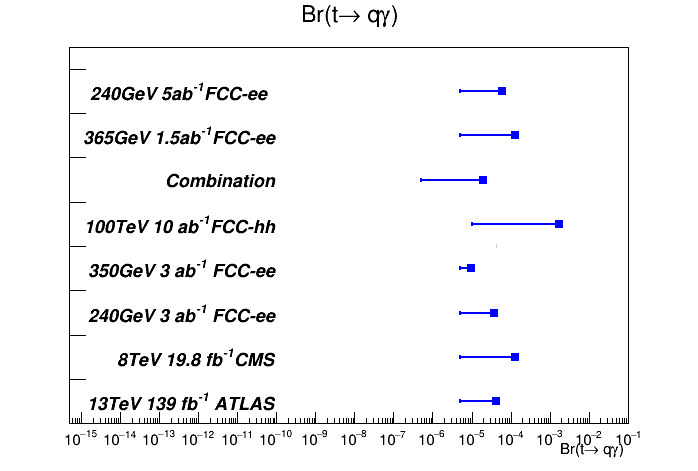
\includegraphics[width=0.5 \textwidth]{tqa_compare.png}	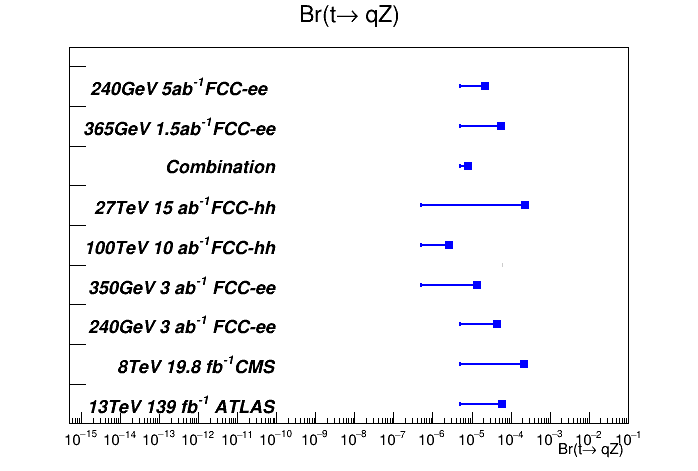
\includegraphics[width=0.5 \textwidth]{tqz_compare.png}
\] 

\end{frame}

%---------------------------------------------------------
%	CLOSING SLIDE
%---------------------------------------------------------
%------------------------------------------------
\section{Summary and Conclusion}
%------------------------------------------------
\begin{frame}
\frametitle{Summary and to do next}
{\bf Summary}
\small
\begin{enumerate}
\item The sensitivity of the FCC-ee to top FCNC interaction is probed by searching $tq$ production.
\item This study has been done in the official FCCAnalysis framework.
\item leptonic decay of the top qurak is considered.
\item We presented the upper limits on the branching ration  for the leptonic (electron $\&$ muon) channel of single-top quark production via FCNC  at two FCC-ee benchmarks ($\sqrt{s}=240$ GeV at 5 ab$^{-1}$ and $\sqrt{s}=365$ GeV at 1.5 ab$^{-1}$).
\item We show the statistical conbination will improve the sensitivity to $tq\gamma$ and $tc\gamma$ couplings.\\
\end{enumerate}
 {\bf To do next}
\begin{enumerate}
\small
\item Applying the mis-tagging efficiency for b-quark.
\item Including hadronic decay channel of top quark.
\item  Statistical combination of leptonic and hadronic decay channel to increase the sensitivity to FCNC interactions.
\item Applying systematic and statistical uncertainties.
\item Using Multivariate analysis to extract the limits.
\end{enumerate}

\end{frame}
\begin{frame}
\[
\includegraphics[width=0.6 \textwidth]{thank3.png}
\] 
\end{frame}

\end{document} 